\part{Inferencia Bayesiana}

\chapter{Inferencia Bayesiana}

\section{Introducción}
La estadistica Bayesiana le debe su nombre al trabajo pionero del reverendo Thomas Bayes titulado "\textit{An Essay towards solving a Problem in the Doctrine of Chances}" publicado póstumamente en 1764 en la "\textit{Philosophical Transactions of the Royal Society of London}". El artículo fue enviado a la Real Sociedad de Londres por Richard Price, amigo de Bayes, en 1763, quién escribió:
\blockquote{"Yo ahora le mando un ensayo que he encontrado entre los papeles de nuestro fallecido amigo Thomas Bayes, y el cual, en mi opinión, tiene un gran mérito, y bien merece ser preservado \ldots En una introducción que él ha escrito para este ensayo, él dice, que su objetivo en un principio fue, descubrir un método por el cual se pueda juzgar la probabilidad de que un evento tenga que ocurrir bajo circunstancias dadas, y bajo la suposición de que nada es conocido sobre dicho evento, salvo que, bajo las mismas circunstancias, éste ha ocurrido un cierto número de veces y fallado otro tanto \ldots Cualquier persona juiciosa verá que el problema aquí mencionado no es de ninguna manera una simple especulación producto de la curiosidad, sino un problema que se necesita resolver para contar con un fundamento seguro para todos nuestros razonamientos concernientes a hechos pasados y a lo que probablemente ocurra de ahí en adelante \ldots El propósito a mí me parece es, mostrar qué razones nosotros tenemos para creer que en la constitución de las cosas existen leyes fijas de acuerdo con las cuales las cosas pasan, y que, por lo tanto, el funcionamiento del mundo debe ser el efecto de la sabiduria y el poder de una causa inteligente, y así, confirmar el argumento tomado desde las causas finales para la existencia de la deidad."}
Aunque la obra de Thomas Bayes data ya de hace más de dos siglos, la estadistica Bayesiana es relativamente nueva, y actualmente ostenta un gran desarrollo aunque no ajeno a también grandes controversias. El marco teórico en el cual se desarrolla la inferencia Bayesiana es idéntico al de la teoría clásica. Se tiene un parámetro poblacional $\theta$ sobre el cual se desen hacer inferencias y se tiene un modelo de probabilidad $f(x/\theta)$ el cual determina la probabilidad de los datos observados r bajo diferentes valores de $\theta$. La diferencia fundamental entre la teoría clásica y la bayesiana está en que $\theta$ es tratado como una cantidad aleatoria. Asi, la inferencia Bayesiana se basa en $f(\theta / x)$ en vez de $f(x/ \theta)$, esto es, en la distribución de probabilidades del parámetro dados los datos.

La inferencia Bayesiana, se puede resumir como el proceso de ajustar un modelo de probabilidad a un conjunto de datos y resumir los resultados me diante una distribución de probabilidades para los parámetros del modelo y para cantidades desconocidas pero observables tales como predicciones para nuevas observaciones. La caracteristica esencial de los métodos Bayesianos está en su uso explícito de probabilidades para cuantificar la incertidumbre en inferencias basadas en el análisis estadístico de los datos. Esto permite un manejo mucho más natural e intuitivo de la inferencia, salvando por ejemplo el problema de la interpretación frecuencial de los resultados. Sin embargo, para hacer uso de un enfoque Bayesiano, es necesario especificar una distribución de probabilidades a priori $f(\theta)$, la cual representa el conocimiento que se tiene sobre la distribución de $\theta$ previo a la obtención de los datos. Esta noción de una distribución a priori para el parámetro constituye el centro del pensamiento Bayesiano y, dependiendo de si se es un defensor o un opositor a esta metodología, su principal ventaja sobre la teoría clásica o su mayor vulnerabilidad.

\section{Teorema de Bayes}

\begin{teo}[de Bayes]
    Sea $(\Omega, \mathcal{A}, P)$ un espacio de probabilidad y sea $A_1, \ldots, A_n \in \mathcal{A}$ una partición de $\Omega$, es decir, $\Omega = \cup_{i=1}^{n} A_i$ y $A_i \cap A_j = \emptyset$ para todo $i \not = j$ y tales que $P(A_i) > 0$ para todo $i$. Sea $B \in \mathcal{A}$ tal que $P(B) > 0$ y tal que  $P(B | A_i)$ son conocidas para todo $i$. Entonces
    \begin{align*}
        P(A_i | B) = \frac{P(B|A_i)P(A_i)}{\sum_{j=1}^{n} P(B|A_j)P(A_j)}, \quad i=1, \ldots,n.
    \end{align*}
\end{teo}
Esta fórmula de conoce como la fórmula de Bayes y
\begin{itemize}
    \item $P(A_j)$ son las \textbf{probabilidades a priori},
    \item $P(B|A_j)$ son las \textbf{verosimilitudes},
    \item $P(A_j|B)$ son las \textbf{probabilidades a posteriori},
\end{itemize}
para todo $j=1 \ldots, n$.

\begin{ejemplo}
    Supogamos que tenemos una caja con una moneda legal, $M_1$, y otra moneda con una cara en cada lado, $M_2$.
    \begin{enumerate}
        \item[a)] Se selecciona una moneda al azar, se lanza y se obtiene cara, ¿qué probabilidad hay de que la moneda elegida sea $M_1$? Sea $C=$''obtener cara''. Tenemos
              \begin{align*}
                   & \underline{\text{Probs a priori}} & \underline{\text{Verosimilitudes}} \\
                   & P(M_1) = \frac{1}{2}              & P(C | M_1) = \frac{1}{2}           \\
                   & P(M_2) = \frac{1}{2}              & P(C | M_2) = 1
              \end{align*}
              Por el Teorema de Bayes
              \begin{align*}
                   & P(M_1 | C) = \frac{\dfrac{1}{2} \cdot \dfrac{1}{2}}{\dfrac{1}{2} \cdot \dfrac{1}{2} + 1 + \dfrac{1}{2}} = \frac{1}{3}, \\
                   & P(M_2 | C) = 1 - P(M_1 | C) = \frac{2}{3}.
              \end{align*}
        \item[b)] Lanzamos de nuevo la moneda elegida y se obtiene otra cara, ¿qué probabilidad hay de que la moneda elegida sea $M_1$? Utilizado el carácter secuencial, tenemos que las probabilidades a posterior de antes pasan a ser nuestras nuevas probabilidades a priori, es decir,
              \begin{align*}
                   & \underline{\text{Probs a priori}} & \underline{\text{Verosimilitudes}} \\
                   & P(M_1|C_1) = \frac{1}{3}          & P(C_2 | M_1) = \frac{1}{2}         \\
                   & P(M_2|C_1) = \frac{2}{3}          & P(C_2 | M_2) = 1
              \end{align*}
              siendo $C_i =$ ''obtener cara en el $i$-ésimo lanzamiento'', $i=1,2$. Por el Teorema de Bayes
              \begin{align*}
                   & P(M_1 | C_1 \cap C_2) = \frac{\dfrac{1}{3} \cdot \dfrac{1}{2}}{\dfrac{1}{3} \cdot \dfrac{1}{2} + 1 + \dfrac{2}{3}} = \frac{1}{5}, \\
                   & P(M_2 | C_1 \cap C_2) = 1 - P(M_1 | C_1 \cap C_2) = \frac{4}{5}.
              \end{align*}
    \end{enumerate}
\end{ejemplo}

\section{Teorema de Bayes generalizado}
Queremos hacer inferencia sobre un parámetro $\theta$ y tenemos una muestra aleatoria simple $x_1,\ldots,x_n$ que sabemos de la población que procede. En la inferencia Bayesiana $\theta$ es una variable aleatoria. Denotamos por $f_{\theta}$ a la \textbf{distribución a priori} de $\theta$. Al igual que en la inferencia clásica, conocemos la \textbf{función de verosimilitud} $L(\vec{x};\theta)$. Mediante el Teorema de Bayes, calculamos $f(\theta | \vec{x})$, que se conoce como \textbf{distribución a posteriori} de $\theta$. Así
\begin{align*}
    f(\theta | \vec{x}) = \frac{f(\vec{x} | \theta) f_{\theta}(\theta)}{f(\vec{x})}. \quad \text{siendo} \quad f(\vec{x}) = \begin{cases}
                                                                                                                                \sum_i f(x_i | \theta_i)f_{\theta_i}(\theta_i),                 & \theta \text{ es discreta}, \\
                                                                                                                                \int_{\Theta} f(\vec{x} | \theta) f_{\theta}(\theta) \ d\theta, & \theta \text{ es continua}.
                                                                                                                            \end{cases}
\end{align*}

\begin{ejemplo}
    Supongamos que tenemos una moneda y queremos estimar la probabilidad de obtener una cara, que denotaremos como $p$. Supongamos que nuestras creencias a priori sobre $p$ se pueden describir con una distribución $U(0,1)$, es decir, todos los valores entre 0 y 1 que puede tomar $p$ son igualmente probables. Realizamos el experimento de tirar la moneda 12 veces y obtenemos 9 caras y 3 cruces. Determinar la distribución a posteriori de $p$.

    Tenemos que
    \begin{align*}
        x | p \sim Ber(p), \quad x = \begin{cases}
                                         1 & \text{si ''sale cara''}, \\
                                         0 & \text{si ''sale cruz''}.
                                     \end{cases}
    \end{align*}
    Es claro que $P(\text{Obtener Cara}) = P(x = 1) = p$. Nos dicen que la distribución a priori de $p$ sigue una $U(0,1)$, así que $f_p(p) = 1$, si $p \in (0,1)$ (y 0 en cualquier otro caso). Sea $x_1,...,x_n$ una muestra aleatoria simple de una $x$. Entonces la función de verosimilitud es
    \begin{align*}
        L(\vec{x};p) & = \prod_{i=1}^{12} f(x_i | p) = \prod_{i=1}^{12} p^{x_i}(1-p)^{1-x_i} p^{\sum_{i=1}^{12} x_i}(1-p)^{12 - \sum_{i=1}^{12} x_i} = p^9(1-p)^3.
    \end{align*}
    Nótese que la útlima igualdad se da porque de los 12 lanzamientos, 9 son caras, por tanto $\sum_{i=1}^{12} x_i = 9$. Finalmente, la distribución a posteriori es
    \begin{align*}
        f(p | \vec{x}) \propto f_p(p)L(\vec{x};p) = p^9(1-p)^3, \quad 0 < p < 1,
    \end{align*}
    de donde concluimos que $p | \vec{x} \sim Be(10,4)$.
\end{ejemplo}

\section{Familias de distribuciones conjugadas}
Son aquellas en las que las distribuciones a priori y a posteriores son de la misma familia.

\subsubsection{Familia conjugada de la Bernoulli}
Consideremos $x | \theta \sim Ber(\theta)$ y supongamos que $\theta \sim Be(p,q)$. Sea $\vec{x} = (x_1,\ldots,x_n)$ nuestro vector de datos. La función de distribución a priori de $\theta$ es $f_{\theta}(\theta) \propto \theta^{p-1}(1-\theta)^{q-1}$, $0 < \theta < 1$. La función de verosimilitud es
\begin{align*}
    L(\vec{x};\theta) = \prod_{i=1}^{n} f(x_i | \theta) \propto \theta^{\sum_{i=1}^{n} x_i}(1-\theta)^{n - \sum_{i=1}^{n} x_i}.
\end{align*}
Finalmente, la función de dsitribución a posteriori es
\begin{align*}
    f(\theta | \vec{x}) \propto f_{\theta}(\theta)L(\vec{x};\theta) \propto \theta^{p + \sum_{i=1}^{n} x_i - 1}(1 - \theta)^{n+q - \sum_{i=1}^{n} x_i -1}.
\end{align*}
Así, hemos llegado a que $\theta | \vec{x} \sim Be\left(p + \sum_{i=1}^{n} x_i, n + q - \sum_{i=1}^{n} x_i \right)$ y por tanto la distribución Beta es una familia conjugada respecto de muestras de la Bernoulli.

\subsubsection{Familia conjugada de la Poisson}
Consideremos $x | \lambda \sim Po(\lambda)$ y supongamos que $\lambda \sim Ga(a,p)$. Sea $\vec{x} = (x_1,\ldots,x_n)$ nuestro vector de datos. La función de distribución a priori de $\lambda$ es
\begin{align*}
    f_{\lambda}(\lambda) = \frac{a^p}{\Gamma(p)}e^{-a\lambda}\lambda^{p-1}, \quad \lambda > 0, \quad a,p > 0.
\end{align*}
La función de verosimilitud es
\begin{align*}
    L(\vec{x};\lambda) = \prod_{i=1}^{n} f(x_i | \lambda) \propto \prod_{i=1}^{n} e^{-\lambda} \lambda^{x_i} = e^{-n \lambda} \lambda^{\sum_{i=1}^{n} x_i}.
\end{align*}
Finalmennte, la función de distribución a posteriori es
\begin{align*}
    f(\lambda | \vec{x}) \propto f_{\lambda}(\lambda)L(\vec{x};\lambda) \propto e^{-(a+n)\lambda} \lambda^{\sum_{i=1}^{n} x_i + p - 1}.
\end{align*}
Así, hemos llegado a que $\lambda | \vec{x} \sim Ga\left(a + n, \sum_{i=1}^{n} x_i + p\right)$ y por tanto la Gamma es una familia conjugada respecto de muestras de la Poisson.

\subsubsection{Familia conjugada de la Normal (media desconocida)}
Consideremos $x | \mu \sim N(\mu,p)$, donde $p = 1/\sigma^2$ es la precisión, y supongamos que $\mu \sim N(m_0,p_0)$. Sea $\vec{x} = (x_1,\ldots,x_n)$ nuestro vector de datos. La función de densidad de $x | \mu$ es
\begin{align*}
    f(x | \mu) = \frac{\sqrt{p}}{\sqrt{2\pi}}e^{-\frac{p}{2}(x-\mu)^2}, \quad x \in \mathbb{R}, \quad \mu \in \mathbb{R}.
\end{align*}
La función de verosimilitud es entonces
\begin{align*}
    L(\vec{x};\mu) = \prod_{i=1}^{n} f(x_i | \mu) \propto \prod_{i=1}^{n} e^{-\frac{p}{2}(x-\mu)^2} \propto e^{-\frac{p}{2}\sum_{i=1}^{n}(x-\mu)^2}
\end{align*}

\begin{obs}
    \begin{align*}
        \sum_{i=1}^{n} (x_i - \mu)^2 & = \sum_{i=1}^{n} (x_i - \overline{x} + \overline{x} - \mu)^2 = \sum_{i=1}^{n} (x_i - \overline{x})^2 n(\overline{x} - \mu)^2 + 2(\overline{x} - \mu)\sum_{i=1}^{n} (x_i - \overline{x}),
    \end{align*}
    pero este último término sabemos que es 0, por tanto
    \begin{align*}
        \sum_{i=1}^{n} (x_i - \mu)^2 = \sum_{i=1}^{n} (x_i - \overline{x})^2 n(\overline{x} - \mu)^2 = (n-1)s^2 + n(\overline{x} - \mu)^2,
    \end{align*}
    siendo
    \begin{align*}
        s^2 = \frac{\sum_{i=1}^{n} (x_i - \overline{x})^2}{n-1}.
    \end{align*}
\end{obs}
Usando esto, llegamos que
\begin{align*}
    L(\vec{x};\mu) \propto e^{-\frac{p}{2}[(n-1)s^2 + (\overline{x} - \mu)^2]} \propto e^{-\frac{p}{2}n(\overline{x} - \mu)^2}.
\end{align*}
La función de distribución a priori es
\begin{align*}
    f_{\mu}(\mu) = \frac{\sqrt{p_0}}{\sqrt{2\pi}} e^{-\frac{p_0}{2}(\mu-m_0)^2} \propto e^{-\frac{p_0}{2}(\mu-m_0)^2}.
\end{align*}
Para calcular la función de distribución a posterior vamos a usar el siguiente Lema.
\begin{lema}
    \begin{align*}
        A(z-a)^2 + B(z-b)^2 = (A+B)\left( z - \frac{Aa + Bb}{A+B} \right)^2 + \frac{AB}{A+B}(a-b)^2
    \end{align*}
\end{lema}
La función de distribución a posterior es
\begin{align*}
    f(\mu | \vec{x}) & \propto f_{\lambda}(\lambda) L(\vec{x} | \mu) \propto e^{-\frac{p_0}{2}(\mu - m_0)} e^{-\frac{p}{2}n(\overline{x} - \mu)^2} = e^{-\frac{1}{2}[p_0(\mu-m_0)^2 + np(\overline{x} - \mu)^2]} \\
                     & = e^{-\frac{1}{2}[a(\mu - b)^2] + c} \propto e^{\frac{-a}{2}(\mu - b)^2},
\end{align*}
que por el Lema anterior, sabemos que
\begin{align*}
    a = p_0 + np, \quad b = \frac{p_0m_0 + np\overline{x}}{p_0 + np}, \quad c = \frac{p_0np}{p_0 + np}(m_0 - x)^2.
\end{align*}
Por tanto,
\begin{align*}
    \mu | \vec{x} \sim N\left(\frac{p_0m_0 + np\overline{x}}{p_0 + np}, p_0 + np\right), \quad p_0 + np \text{ es la precisón},
\end{align*}
y por tanto, la Normal es una familia conjugada respecto de muestras de la Normal con media desconocida y precisión conocida.

\subsubsection{Familia conjugada de la Normal (precisión desconocida)}
Consideremos $x | \tau \sim N(\mu,\tau)$, donde $\tau = 1/\sigma^2$ es la precisión, y supongamos que $\tau \sim Ga(a_0,p_0)$. Sea $\vec{x} = (x_1,\ldots,x_n)$ nuestro vector de datos. Tenemos que
\begin{align*}
     & f(x |\tau) = \frac{\sqrt{\tau}}{\sqrt{2\pi}}e^{-\frac{\tau}{2}(x -\mu)^2}, \quad x \in \mathbb{R}, \tau > 0, \\
     & f_{\tau}(\tau) = \frac{a_0^{p_0}}{\Gamma(p_0)}e^{-a_0 \tau}\tau^{p_0-1}.
\end{align*}
La función de verosimilitud es entonces
\begin{align*}
    L(\vec{x};\tau) = \prod_{i=1}^{n} f(x_i | \tau) \propto \prod_{i=1}^{n} \sqrt{\tau} \exp\left[-\frac{\tau}{2}(x_i - \mu)\right] = \tau^{\frac{n}{2}}\exp\left[-\frac{\tau}{2} \sum_{i=1}^{n}(x_i -\mu)^2\right].
\end{align*}
La función de distribución a posteriori es
\begin{align*}
    f(\tau | \vec{x}) \propto f_{\tau}(\tau) L(\vec{x} | \tau) = \tau^{\frac{n}{2} + p_0 -1} \exp\left[ - \tau \left( a_0 + \frac{1}{2} \sum_{i=1}^{n}(x_i-\mu)^2 \right) \right].
\end{align*}
Así, hemos llegado a que $\tau | \vec{x} \sim Ga(a_n,p_n)$, siendo
\begin{align*}
    a_n = a_0 + \frac{1}{2} \sum_{i=1}^{n} (x_i - \mu)^2, \quad p_n = \frac{n}{2} + p_0.
\end{align*}
Por tanto, la Gamma es una familia conjugada respecto de muestras de la Normal con media conocida y precisión desconocida.

\begin{defi}
    Si $X \sim Ga(a,p)$ y definimos $Y = 1/X$, entonces $Y \sim  GaI(a,p)$.
\end{defi}
Calculemos la función de densidad de $Y \sim  GaI(a,p)$. Sabemos que la densidad de $X \sim Ga(a,p)$ es
\begin{align*}
    f_X(x) = \frac{a^p}{\Gamma(p)} e^{-ax}x^{p-1}, \quad x >0, a,p>0.
\end{align*}
Tenemos que $Y = 1/X$, es decir, $X = 1/Y$. Aplicando el Teorema de cambio de variable, tenemos que la densidad de $Y$ es
\begin{align*}
    f_Y(y) & = f_X\left( \frac{1}{y} \right) \left| \frac{d}{dy} \left( \frac{1}{y} \right) \right| = \frac{a^p}{\Gamma(p)} e^{-a/y} \left( \frac{1}{y} \right)^{p-1} \frac{1}{y^2}
    = \frac{a^p}{\Gamma(p)}  e^{-a/y} y^{-(p+1)}, \quad y > 0.
\end{align*}

\subsubsection{Familia conjugada de la Normal (varianza desconocida)}
Consideremos $x | \sigma^2 \sim N(\mu,\sigma^2)$ y supongamos que $\sigma^2 \sim GaI(a_0,p_0)$. Sea $\vec{x} = (x_1,\ldots,x_n)$ nuestro vector de datos. Tenemos que
\begin{align*}
     & f(x | \sigma^2) = \frac{1}{\sqrt{2\pi \sigma^2}} e^{- \frac{1}{2\sigma^2}(x -\mu)^2}, \quad x \in \mathbb{R}, \sigma^2 > 0, \\
     & f_{\sigma^2}(\sigma^2) = \frac{a_0^{p_0}}{\Gamma(p_0)} \left(\sigma^2\right)^{-(p_0+1)}, \quad a_0,p_0 > 0.
\end{align*}
La función de verosimilitud es entonces
\begin{align*}
    L(\vec{x}; \sigma^2) =  \prod_{i=1}^{n} f(x_i | \sigma^2) \propto \prod_{i=1}^{n} \frac{1}{\sqrt{\sigma^2}} e^{- \frac{1}{2\sigma^2}(x -\mu)^2} = \left(\sigma^2 \right)^{-\frac{n}{2}} \exp\left[ - \frac{1}{2\sigma^2} \sum_{i=1}^{n} (x_i - \mu)^2 \right].
\end{align*}
La función de distribución a posteriori es
\begin{align*}
    f(\sigma^2 | \vec{x}) \propto f_{\sigma^2}(\sigma^2) L(\vec{x} | \sigma^2) \propto \left(\sigma^2 \right)-(p_0 + n/2 + 1) \exp\left[- \frac{1}{\sigma^2}\left( a_0 + \frac{1}{2} \sum_{i=1}^{n} (x_i - \mu)^2\right)\right].
\end{align*}
Así, hemos llegado a que $\sigma^2 | \vec{x} \sim GaI(a_n,p_n)$, siendo
\begin{align*}
    a_n = a_0 + \frac{1}{2} \sum_{i=1}^{n} (x_i - \mu)^2, \quad p_n = p_0 + \frac{n}{2}.
\end{align*}
Por tanto, la Gamma Inversa es una familia conjugada respecto de muestras de la Normal con media conocida y varianza desconocida.

\begin{defi}
    Decimos que $(\mu, \tau) \sim NGa(m_0, \tau_0, a_0, p_0)$ (Normal-Gamma) siendo $m_0 \in \mathbb{R}$, $\tau_0,a_0,p_0 > 0$ si
    \begin{align*}
        \mu | \tau & \sim N(m_0, \tau \tau_0), \quad \mu \in \mathbb{R}, \\
        \tau       & \sim Ga(a_0,p_0), \quad \tau > 0.
    \end{align*}
\end{defi}
Calculemos la función de densidad de $(\mu, \tau) \sim NGa(m_0, \tau_0, a_0, p_0)$. Tenemos que
\begin{align*}
     & f(\mu | \tau) = \frac{\sqrt{\tau \tau_0}}{\sqrt{2\pi}} e^{- \frac{\tau \tau_0}{2}(\mu - m_0)^2}, \quad \mu \in \mathbb{R}, \\
     & f_{\tau}(\tau) = \frac{a_0^{p_0}}{\Gamma(p_0)} e^{-a_0\tau} \tau^{p_0-1}, \quad \tau > 0.
\end{align*}
Así,
\begin{align*}
    f(\mu,\tau) = f(\mu | \tau) f_{\tau}(\tau) = \frac{\sqrt{ \tau_0}}{\sqrt{2\pi}} \frac{a_0^{p_0}}{\Gamma(p_0)} \tau^{p_0 - 1/2} e^{-\tau\left( a_0 + \frac{\tau_0}{2}(\mu - m_0)^2 \right)}.
\end{align*}
Podemos darle una vuelta a la definición anterior de la siguiente manera
\begin{defi}
    Decimos que $(\mu, \tau) \sim NGa(m_0, \tau_0, a_0, p_0)$ (Normal-Gamma) si
    \begin{align*}
        \frac{\sqrt{\tau \tau_0}}{\sqrt{2\pi}} \frac{a_0^{p_0}}{\Gamma(p_0)} \tau^{p_0 - 1/2} e^{-\tau\left( a_0 + \frac{\tau_0}{2}(\mu - m_0)^2 \right)},
    \end{align*}
    siendo  $\mu \in \mathbb{R}$, $\tau > 0$, $m_0 \in \mathbb{R}$, $\tau_0,a_0,p_0 > 0$.
\end{defi}
Recordemos que la función de densidad de la $t$-Student  con $n$ grados de libertad es
\begin{align*}
    f_T(t) = \frac{\Gamma\left( \frac{n+1}{2} \right)}{\Gamma\left( \frac{1}{2} \right)\Gamma\left( \frac{n}{2} \right)\sqrt{n}} \left(1 + \frac{t^2}{n} \right)^{-\frac{n+1}{2}}, \quad t \in \mathbb{R}.
\end{align*}
Además,
\begin{align*}
    E[T] = 0, \quad \text{si $ n > 1$}, \quad Var[T] = \frac{n}{n-2}, \quad \text{si $n >2$}.
\end{align*}
Ahora vamos a generalizar la distribución $t$-Student, permitiendo desplazarla (cambiar la media) y aplastarla (cambiar la ''varianza'')
\begin{defi}
    Si $T \sim t_n$, entonces $X = \mu + \frac{1}{\sqrt{p}}T \sim t(\mu,p,n)$.
\end{defi}
Tenemos que
\begin{align*}
    E[X]   & = E\left[\mu + \frac{1}{\sqrt{p}}T \right] = \mu + \frac{1}{\sqrt{p}} E[T] = \mu,                    \\
    Var[X] & =  Var\left[\mu + \frac{1}{\sqrt{p}}T \right] = \frac{1}{p}Var[T] = \frac{1}{p} \cdot \frac{n}{n-2}.
\end{align*}
Llamaremos \textit{precisión} de $X$ a
\begin{align*}
    \text{precisión($X$)} = \frac{1}{p} \cdot \frac{n}{n-2}.
\end{align*}
Calculemos ahora la función de densidad de $X$. Tenemos que
\begin{align*}
    X = \mu + \frac{1}{\sqrt{p}}T \Longleftrightarrow T = \sqrt{p}(X - \mu).
\end{align*}
Aplicando el Teorema de cambio de variable
\begin{align*}
    f_X(x) & = f_T\left( \sqrt{p} (x - \mu) \right) \left| \frac{d}{dx} \left( \sqrt{p}(x -\mu) \right) \right|
    = \frac{\Gamma\left( \frac{n+1}{2} \right)\sqrt{p}}{\Gamma\left( \frac{1}{2} \right)\Gamma\left( \frac{n}{2} \right)\sqrt{n}} \left(1 + \frac{p(x-\mu)^2}{n} \right)^{-\frac{n+1}{2}}, \quad x \in \mathbb{R}.
\end{align*}

\begin{obs} \
    \begin{itemize}
        \item $t_1$ es la conocida distribución de Cauchy.
        \item $t_n \xrightarrow[]{n \to \infty} N(0,1)$.
    \end{itemize}
\end{obs}

\begin{teo}
    Si $(\mu, \tau) \sim NGa(m_0,\tau_0,a_0,p_0)$, entonces
    \begin{align*}
        \mu \sim t\left(m_0,  \frac{\tau_0p_0}{2},2p_0 \right).
    \end{align*}
\end{teo}

\begin{obs}
    Si tenemos que $\mu | \tau \sim N(0,\tau)$ y $\tau \sim Ga\left( \frac{n}{2},\frac{n}{2}\right)$, entonces $\mu \sim t(0,1,n) \equiv t_n$ (Génesis Bayesiana de la $t$-Student).

    Además, si $\mu | \sigma^2 \sim N(\mu,\sigma^2)$ y $\sigma^2 \sim GaI\left( \frac{n}{2}, \frac{n}{2} \right)$, entonces $\mu \sim t_n$.
\end{obs}

\subsubsection{Familia conjugada de la Normal (media y precisión desconocidas)}
Consideremos $x | \mu,\tau \sim N(\mu,\sigma^2)$, siendo $\tau = 1/\sigma^2 $ es la precisión y supongamos que
\begin{align*}
    (\mu,\tau) \sim NGa(m_0,\tau_0,a_0,p_0).
\end{align*}

Sea $\vec{x} = (x_1,\ldots,x_n)$ nuestro vector de datos. Tenemos que
\begin{align*}
     & f(\mu,\tau) = \frac{\sqrt{\tau_0}}{\sqrt{2\pi}} \frac{a_0^{p_0}}{\Gamma(p_0)} \tau^{p_0 - 1/2} e^{-\tau\left( a_0 + \frac{\tau_0}{2}(\mu - m_0)^2 \right)}, \\
     & f(x | \mu, \tau) = \frac{\tau}{\sqrt{2\pi}} e^{-\frac{\tau}{2}(x-\mu)^2}, \quad x \in \mathbb{R}, \mu \in \mathbb{R}, \tau \ge 0.
\end{align*}
La función de verosimilitud es entonces
\begin{align*}
    L(\vec{x};\mu,\tau) = \prod_{i=1}^{n}f(x_i | \mu, \tau) \propto \tau^{\frac{n}{2}}\exp\left[ - \frac{\tau}{2} \sum_{i=1}^{n} (x_i - \mu)^2\right]
    = \tau^{\frac{n}{2}} e^{ (n-1)s^2 + n(\overline{x} -\mu)^2 },
\end{align*}
donde
\begin{align*}
    s^2 = \frac{\sum_{i=1}^{n} (x_i - \overline{x})^2}{n-1}.
\end{align*}
La fución de distribución a posteriori es
\begin{align*}
    f(\mu,\tau | \vec{x}) \propto f(\mu,\tau) L(\vec{x};\mu,\tau) \propto \ldots \propto \tau^{n/2 - p_0 - 1/2} e^{-\frac{\tau}{2}(2a_0 + (n-1)s^2 + a(\mu - b)^2) + c)},
\end{align*}
siendo
\begin{align*}
    a = \tau_0 + n, \quad b = \frac{\tau_0 m_0 + n \overline{x}}{\tau_0 + n}, \quad c = \frac{\tau_0n}{\tau_0 + n}(\overline{x} - m_0)^2.
\end{align*}
Así, hemos llegado a que $(\mu,\tau) | \vec{x} \sim NGa \left(b, a, \frac{2a_0 + (n-1)s^2 + c}{2}, \frac{n}{2} + p_0 \right)$, es decir,
\begin{align*}
    (\mu,\tau) | \vec{x} \sim NGa(m_n, \tau_n, a_n,p_n),
\end{align*}
siendo
\begin{align*}
    m_n = \frac{\tau_0 m_0 + n \overline{x}}{\tau_0 + n}, \quad \tau_n = \tau_0 + n, \quad a_n = \frac{2a_0 + (n-1)s^2 + \frac{\tau_0n}{\tau_0 + n}(\overline{x} - m_0)^2}{2}, \quad p_n = \frac{n}{2} + p_0.
\end{align*}
Por tanto, la Normal-Gamma es una familia conjugada respecto de muestras de la Normal con media y precisión desconocidas.

\section{Distribuciones a priori no informativas}
Se deducen de la regla de Jeffreys:
\begin{align*}
    f_{\theta}(\theta) \propto \sqrt{J(\theta)}, \quad J(\theta) = - E \left[ \frac{\partial^2 \log f(x | \theta)}{\partial \theta^2} \right].
\end{align*}
$J(\theta)$ se conoce como \textit{información de Fisher}. Es importante saber que la regla de Jeffreys no siempre proporiciona funciones de densidad, en realidad, proporciona densidades impropias.
\begin{obs}
    En la asignatura de Inferencia Estadística vimos que si $\widehat{\theta}$ es un estimador insesgado para $\theta$, entonces
    \begin{align*}
        Var[ \widehat{\theta}] = \frac{1}{J( \widehat{\theta})},
    \end{align*}
    que se conoce como la Cota de Frechet-Cramer-Rao.
\end{obs}

\subsubsection{Distribución no informativa de la Bernoulli}
Supongamos que $x | \theta \sim Ber(\theta)$. Entonces
\begin{align*}
    f(x | \theta)                                           & = \theta^x(1-\theta)^{1-x}, \quad x=0,1, \quad 0 < \theta < 1, \\
    \log f(x | \theta)                                      & = x \log \theta + (1 - x) \log (1 -\theta),                    \\
    \frac{\partial \log f(x | \theta)}{\partial \theta}     & = \frac{x}{\theta} - \frac{1-x}{1-\theta},                     \\
    \frac{\partial^2 \log f(x | \theta)}{\partial \theta^2} & = - \frac{x}{\theta^2} - \frac{1-x}{(1-\theta)^2}.
\end{align*}
Entonces, la información de Fisher es
\begin{align*}
    J(\theta) & = E \left[ \frac{x}{\theta^2} + \frac{1-x}{(1-\theta)^2}\right] = \frac{1}{\theta} E[x] + \frac{1}{(1-\theta)^2}E[1-x] = \frac{1}{\theta^2}\theta + \frac{1}{(1-\theta)^2}(1-\theta) \\
              & = \frac{1}{\theta} + \frac{1}{1-\theta} = \frac{1}{\theta(1-\theta)}
\end{align*}
Así, la regla de Jeffreys nos dice que
\begin{align*}
    f_{\theta}(\theta) \propto \sqrt{J(\theta)} = \sqrt{\frac{1}{\theta(1-\theta)}} = \theta^{-1/2}(1-\theta)^{-1/2}.
\end{align*}
De donde deducimos que $\theta \sim Be\left( \frac{1}{2}, \frac{1}{2} \right)$.

\subsubsection{Distribución no informativa de la Poisson}
Supongamos que $x | \lambda \sim Po(\lambda)$. Entonces
\begin{align*}
    f(x | \lambda)                                            & = \frac{e^{-\lambda}\lambda^x}{x!} \propto e^{-\lambda}\lambda^x, \quad x \in \mathbb{N} \cup \{0\}, \quad\lambda >0, \\
    \log f(x | \lambda)                                       & \propto -\lambda + x \log \lambda ,                                                                                   \\
    \frac{\partial \log f(x | \lambda)}{\partial \lambda}     & \propto - 1 + \frac{x}{\lambda},                                                                                      \\
    \frac{\partial^2 \log f(x | \lambda)}{\partial \lambda^2} & \propto - \frac{x}{\lambda^2} .
\end{align*}
Entonces, la información de Fisher es
\begin{align*}
    J(\lambda) & \propto E\left[ \frac{x}{\lambda^2} \right] = \frac{1}{\lambda^2}E[x] = \frac{1}{\lambda^2} \lambda = \frac{1}{\lambda}.
\end{align*}
Así, la regla de Jeffreys nos dice que
\begin{align*}
    f_{\lambda}(\lambda) \propto \sqrt{J(\lambda)} \propto \sqrt{\frac{1}{\lambda}} = \lambda^{-1/2}.
\end{align*}

\subsubsection{Distribución no informativa de la Normal (media desconocida)}
Supongamos que $x | \mu \sim N(\mu,p)$, siendo $p = 1/\sigma^2$ la precisión. Entonces
\begin{align*}
    f(x | \mu)                                        & = \frac{\sqrt{p}}{\sqrt{2\pi}}e^{-\frac{p}{2}(x-\mu)^2} \propto e^{-\frac{p}{2}(x-\mu)^2} \\
    \log f(x | \mu)                                   & \propto -\frac{p}{2}(x-\mu)^2  ,                                                          \\
    \frac{\partial \log f(x | \mu)}{\partial \mu}     & \propto p(x-\mu),                                                                         \\
    \frac{\partial^2 \log f(x | \mu)}{\partial \mu^2} & \propto -p \propto -1 .
\end{align*}
Entonces, la información de Fisher es
\begin{align*}
    J(\mu) & \propto E\left[ 1 \right] = 1.
\end{align*}
Así, la regla de Jeffreys nos dice que
\begin{align*}
    f_{\mu}(\mu) \propto \sqrt{J(\mu)} \propto 1.
\end{align*}

\subsubsection{Distribución no informativa de la Normal (desviación típica desconocida)}
Supongamos que $x | \sigma \sim N(\mu,\sigma)$. Entonces
\begin{align*}
    f(x | \sigma)                                           & = \frac{1}{\sqrt{2\pi\sigma^2}}e^{-\frac{1}{2\sigma^2}(x-\mu)^2} \propto \frac{1}{\sigma} e^{-\frac{1}{2\sigma^2}(x-\mu)^2} \\
    \log f(x | \sigma)                                      & \propto - \log \sigma - \frac{1}{2\sigma^2}(x-\mu)^2   ,                                                                    \\
    \frac{\partial \log f(x | \sigma)}{\partial \sigma}     & \propto - \frac{1}{\sigma} + \frac{(x-\mu)^2}{\sigma^3}                                                                     \\
    \frac{\partial^2 \log f(x | \sigma)}{\partial \sigma^2} & \propto \frac{1}{\sigma^2} - \frac{3(x-\mu)^2}{\sigma^4} .
\end{align*}
Entonces, la información de Fisher es
\begin{align*}
    J(\sigma) & \propto E\left[ -\frac{1}{\sigma^2} + \frac{3(x-\mu)^2}{\sigma^4} \right] \propto -\frac{1}{\sigma^2} + \frac{3}{\sigma^4} E\left[ (x-\mu)^2\right] = - \frac{1}{\sigma^2} + \frac{3}{\sigma^4}\sigma^2 \propto \frac{1}{\sigma^2}.
\end{align*}
Así, la regla de Jeffreys nos dice que
\begin{align*}
    f_{\sigma}(\sigma) \propto \sqrt{J(\sigma)} \propto \sqrt{\frac{1}{\sigma^2}} = \frac{1}{\sigma}.
\end{align*}

\subsubsection{Distribución no informativa de la Normal (desviación típica desconocida)}
Supongamos que $x | \sigma^2 \sim N(\mu,\sigma^2)$. En lugar de repetir todo el proceso anterior, podemos hacer lo siguiente. Definimos $x = \sigma$ e $y = \sigma^2$. Es claro que $y = x^2$, es decir, $x = \sqrt{y}$. Acabamos de probar que $f_{x}(x) \propto 1/x$. Usando el Teoremas de cambio de variables
\begin{align*}
    f_y(y) = f_x\left( \sqrt{y} \right) \left| \frac{d}{dy} \left( \sqrt{y} \right) \right| \propto \frac{1}{\sqrt{y}} \cdot \frac{1}{2\sqrt{y}} \propto \frac{1}{y}.
\end{align*}
Así,
\begin{align*}
    f_{\sigma^2}(\sigma^2) \propto \frac{1}{\sigma^2}.
\end{align*}

\subsubsection{Distribución no informativa de la Normal (precisión desconocida)}
Supongamos que $x | \tau \sim N(\mu,\tau)$, siendo $\tau = 1/\sigma^2$ la precisión. En lugar de repetir todo el proceso anterior, podemos hacer lo siguiente. Definimos $x = \sigma$ e $y = 1/\sigma^2$. Es claro que $y = 1/x^2$, es decir, $x = 1/\sqrt{y}$. Ya hemos probado que $f_{x}(x) \propto 1/x$. Usando el Teoremas de cambio de variables
\begin{align*}
    f_y(y) = f_x\left( 1/\sqrt{y} \right) \left| \frac{d}{dy} \left( 1/\sqrt{y} \right) \right| \propto \sqrt{y} \cdot \frac{2}{y\sqrt{y}} \propto \frac{1}{y}.
\end{align*}
Así,
\begin{align*}
    f_{\tau}(\tau) \propto \frac{1}{\tau}.
\end{align*}

\subsubsection{Distribución no informativa de la Normal (media y desviación típicas desconocidas)}
Supongamos que $x | \mu,\sigma \sim N(\mu,\sigma)$. Entonces
\begin{align*}
    f(\mu,\sigma) = f_{\mu}(\mu) \cdot f_{\sigma}(\sigma) \propto \frac{1}{\sigma}.
\end{align*}

\subsubsection{Distribución no informativa de la Normal (media y varianza desconocidas)}
Supongamos que $x | \mu,\sigma^2 \sim N(\mu,\sigma^2)$. Entonces
\begin{align*}
    f(\mu,\sigma^2) = f_{\mu}(\mu) \cdot f_{\sigma^2}(\sigma^2) \propto \frac{1}{\sigma^2}.
\end{align*}
\subsubsection{Distribución no informativa de la Normal (media y precisión desconocidas)}
Supongamos que $x | \mu,\tau \sim N(\mu,\tau)$, siendo $\tau = 1/\sigma^2$ la precisión. Entonces
\begin{align*}
    f(\mu,\tau) = f_{\mu}(\mu) \cdot f_{\tau}(\tau) \propto \frac{1}{\tau}.
\end{align*}

\tcbsetforeverylayer{colframe=yellow!90!black}
\begin{tcolorbox}[title=Regla de Oro]
    Todo sale de la distribución a priori.
\end{tcolorbox}

\section{Estimación puntual}
La estimación puntual Bayesiana es un problema de decisión. Debemos tener una función de pérdida, $L : \Theta \times \Theta \longrightarrow \mathbb{R}$, siendo $L(\theta,t)$ la pérdida si estimamos el parámetro por $t$ siendo $\theta$ su verdadero valor. Las funciones de pérdida más usuales son:
\begin{itemize}
    \item Función de pérdida cuadrática: $L(\theta,t) = (\theta - t)^2$.
    \item Función pérdida de valor absoluto: $L(\theta,t) = |\theta - t|$.
    \item Función de pérdida 0-1:
          \begin{align*}
              L(\theta,t) = \begin{cases}
                                0, & |\theta - t| \leq \varepsilon, \\
                                1, & |\theta - t| > \varepsilon.
                            \end{cases}
          \end{align*}
\end{itemize}
Lo ideal sería minimizar esta función, pero $\theta$ es desconocido. Así que, minimizamos $E[L(\theta,t) | \vec{x}]$, siendo $\vec{x}$ nuestros datos. Elegimos $\widehat{\theta}$ tal que
\begin{align*}
    E[L(\theta, \widehat{\theta})] = \min_{t} E[L(\theta,t) | \vec{x}] = \min_t \int_{\Theta} L(\theta,t) f(\theta | \vec{x}) \ d\theta.
\end{align*}
Supongamos que tenemos como función de pérdida $L(\theta,t) = (\theta - t)^2$. Entonces
\begin{align*}
    \psi(t) & = E[L(\theta,t) | \vec{x}] = \int_{\Theta} (\theta - t)^2 f(\theta | \vec{x}) \ d\theta                                                                          \\
            & = \int_{\Theta} \theta^2 f(\theta | \vec{x}) \ d\theta + t^2 \int_{\Theta} f(\theta | \vec{x}) \ d\theta - 2t \int_{\Theta} \theta f(\theta | \vec{x}) \ d\theta \\
            & = \int_{\Theta} \theta^2 f(\theta | \vec{x}) \ d\theta + t^2 - 2tE[\theta | \vec{x}]
\end{align*}
Calculemos el mínimo de $\psi$ (respecto de $t$).
\begin{align*}
    \psi'(t) = 2t - 2E[\theta | \vec{x}] \Longrightarrow \psi'(t) = 0 \Longleftrightarrow t = E[\theta | \vec{x}]
\end{align*}
Se comprueba facilmente que, efectivamente, es un mínimo. Por tanto, tomamos $\widehat{\theta} = E[\theta | \vec{x}]$, es decir, el estimador Bayesiano de $\theta$ bajo la función de pérdida cuadrática es la media a posteriori de $\theta$, es decir, $E[\theta | \vec{x}]$.

Si repitiésemos esto para las otras funciones de pérdida, llegaríamos a que
\begin{itemize}
    \item El estimador Bayesiano de $\theta$ bajo la función de pérdida de valor absoluto es la mediana a posteriori de $\theta$.
    \item El estimador Bayesiano de $\theta$ bajo la función de pérdida 0-1 es la moda a posteriori de $\theta$.
\end{itemize}

\begin{obs}
    Se puede probar que la media a posteriori es una media ponderada de la media a priori y del estimador de máxima verosimilitud, es decir, existe $\omega \in (0,1)$ tal que
    \begin{align*}
        E[\theta | \vec{x}] = \omega E[\theta] + (1 - \omega) \widehat{\theta}_{EMV}
    \end{align*}
\end{obs}

\section{Intervalos de credibilidad}

\begin{defi}
    Un intervalo de credibilidad para $\theta$ de contenido probabilístico $1 - \alpha$, es un intervalo $(a,b)$ tal que
    \begin{align*}
        P(a < \theta | \vec{x} < b) = 1 - \alpha.
    \end{align*}
\end{defi}

\begin{defi}
    Una región $R$ es de máxima densidad a posteriori (MDP) de $\theta$ de contenido probabilístico $1-\alpha$, si
    \begin{enumerate}
        \item $P(\theta | \vec{x} \in R) = 1 - \alpha$.
        \item Si $\theta_1 \in R$ y $\theta_2 \not \in R$, entonces $f(\theta_1 | \vec{x}) > f(\theta_2 | \vec{x})$.
    \end{enumerate}
\end{defi}

\begin{obs}
    Si la distribución de $\theta | \vec{x}$ es unimodal, la región MDP de contenido probabilistico $1-\alpha$ para $\theta$ es un intervalo $(a,b)$ tal que
    \begin{enumerate}
        \item $P(a < \theta | \vec{x} < b) = 1 - \alpha$.
        \item $f(a | \vec{x}) = f(b | \vec{x})$.
    \end{enumerate}
\end{obs}

\section{Contrastes de hipótesis}
Los posibles contrastes de hipótesis que plantearemos serán los siguientes:
\begin{align*}
    1. \begin{cases}
           H_0 : \theta \leq \theta_0 \\
           H_1 : \theta > \theta_0
       \end{cases} \quad     2.\begin{cases}
                                   H_0 : \theta \ge \theta_0 \\
                                   H_1 : \theta < \theta_0
                               \end{cases} \quad     3.\begin{cases}
                                                           H_0 : \theta = \theta_0 \\
                                                           H_1 : \theta \not = \theta_0
                                                       \end{cases}
\end{align*}
Resolveremos estos contrastes de la siguiente manera
\begin{enumerate}
    \item Calculamos $P(H_0 | \vec{x}) = P(\theta \leq \theta_0 |\vec{x})$ y $P(H_1 | \vec{x}) = P(\theta > \theta_0 | \vec{x})$.
          \begin{itemize}
              \item Si $P(H_0 | \vec{x}) > P(H_1 | \vec{x})$, aceptamos $H_0$.
              \item Si $P(H_0 | \vec{x}) \leq P(H_1 | \vec{x})$, rechazamos $H_0$.
          \end{itemize}
    \item Calculamos $P(H_0 | \vec{x}) = P(\theta \ge \theta_0 |\vec{x})$ y $P(H_1 | \vec{x}) = P(\theta < \theta_0 | \vec{x})$.
          \begin{itemize}
              \item Si $P(H_0 | \vec{x}) > P(H_1 | \vec{x})$, aceptamos $H_0$.
              \item Si $P(H_0 | \vec{x}) \leq P(H_1 | \vec{x})$, rechazamos $H_0$.
          \end{itemize}
    \item Fijamos nivel de significación $\alpha$.
          \begin{itemize}
              \item Si $\theta_0 \in MDP_{1 - \alpha}(\theta | \vec{x})$, aceptamos $H_0$ a nivel de significación $\alpha$.
              \item Si $\theta_0 \not\in MDP_{1 - \alpha}(\theta | \vec{x})$, rechazamos $H_0$ a nivel de significación $\alpha$.
          \end{itemize}
\end{enumerate}

\section{Distribución predictiva}
Supongamos que $\vec{x} = (x_1, \ldots, x_n)$ es nuestro vector de datos y supongamos que queremos predecir una nueva observación $x_{n+1}$.
\begin{align*}
    f(x_{n+1} | \vec{x}) = \int_{\Theta} f(x_{n+1} | \theta) f(\theta | \vec{x}) \ d\theta.
\end{align*}
\begin{ejemplo}

\end{ejemplo}

\section{Análisis Bayesiano para datos de Bernoulli}
Supongamos que $x | \theta \sim Ber(\theta)$ y sea $\vec{x} = (x_1, \ldots, x_n)$ nuestro vector de datos.

\subsubsection{Caso informativo}
Ya habiamos calculado la familia conjugada para muestras de la Bernoulli y vimos que
\begin{align*}
    \theta           & \sim Be(p,q),                                                             \\
    \theta | \vec{x} & \sim Be\left( \sum_{i=1}^{n} x_i + p, n - \sum_{i=1}^{n} x_i + q \right).
\end{align*}

\underline{Estimación puntual}
\begin{itemize}
    \item Si $L(\theta,t)$ es la función de pérdida cuadrática,
          \begin{align*}
              \widehat{\theta} = E[\theta |  \vec{x}] = \frac{\sum_{i=1}^{n} x_i + p}{n + p + q}.
          \end{align*}
    \item Si $L(\theta,t)$ es la función de pérdida de valor absoluto, $\widehat{\theta} = Me[\theta | \vec{x}]$.
    \item Si $L(\theta,t)$ es la función de pérdida 0-1,
          \begin{align*}
              \widehat{\theta} = Mo[\theta | \vec{x}] = \frac{\sum_{i=1}^{n} x_i + p}{n + p + q - 2}.
          \end{align*}
\end{itemize}
Calculemos $\omega \in (0,1)$ tal que
\begin{align*}
    E[\theta | \vec{x}]                      & = \omega E[\theta] + (1 - \omega) \widehat{\theta}_{EMV}          \\
    \frac{\sum_{i=1}^{n} x_i + p}{n + p + q} & = \omega \frac{p}{p+q} + (1-\omega) \frac{\sum_{i=1}^{n} x_i}{n}.
\end{align*}
Es fácil comprobar que $\omega = \frac{p+q}{n+p+q}$. Observamos que $\omega \xrightarrow[n \to \infty]{} 0$, lo que nos dice que cuantos más datos tenemos, el estimador de máxima verosimilitud de $\theta$ tiene más peso.

\underline{Intervalos de credibilidad}: Un intervalo de credibilidad de contenido probabilístico $1-\alpha$ es un intervalo $(a,b)$ tal que
\begin{align*}
    1 - \alpha = P(a < \theta | \vec{x} < b) = \int_{a}^{b} f(\theta | \vec{x}) \ d\theta.
\end{align*}
El intervalo MDP de contenido probabilístico $1-\alpha$ es un intervalo $(a,b)$ tal que
\begin{enumerate}
    \item $P(a < \theta | \vec{x} < b) = 1 - \alpha$.
    \item $f(a | \vec{x}) = f(b | \vec{x})$.
\end{enumerate}
\underline{Contrastes de hipótesis}
\begin{align*}
    1. \begin{cases}
           H_0 : \theta \leq \theta_0 \\
           H_1 : \theta > \theta_0
       \end{cases} \quad     2.\begin{cases}
                                   H_0 : \theta \ge \theta_0 \\
                                   H_1 : \theta < \theta_0
                               \end{cases} \quad     3.\begin{cases}
                                                           H_0 : \theta = \theta_0 \\
                                                           H_1 : \theta \not = \theta_0
                                                       \end{cases}
\end{align*}

\begin{enumerate}
    \item Calculamos $P(H_0 | \vec{x}) = P(\theta \leq \theta_0 |\vec{x})$ y $P(H_1 | \vec{x}) = P(\theta > \theta_0 | \vec{x})$.
          \begin{itemize}
              \item Si $P(H_0 | \vec{x}) > P(H_1 | \vec{x})$, aceptamos $H_0$.
              \item Si $P(H_0 | \vec{x}) \leq P(H_1 | \vec{x})$, rechazamos $H_0$.
          \end{itemize}
    \item Calculamos $P(H_0 | \vec{x}) = P(\theta \ge \theta_0 |\vec{x})$ y $P(H_1 | \vec{x}) = P(\theta < \theta_0 | \vec{x})$.
          \begin{itemize}
              \item Si $P(H_0 | \vec{x}) > P(H_1 | \vec{x})$, aceptamos $H_0$.
              \item Si $P(H_0 | \vec{x}) \leq P(H_1 | \vec{x})$, rechazamos $H_0$.
          \end{itemize}
    \item Fijamos nivel de significación $\alpha$.
          \begin{itemize}
              \item Si $\theta_0 \in MDP_{1 - \alpha}(\theta | \vec{x})$, aceptamos $H_0$ a nivel de significación $\alpha$.
              \item Si $\theta_0 \not\in MDP_{1 - \alpha}(\theta | \vec{x})$, rechazamos $H_0$ a nivel de significación $\alpha$.
          \end{itemize}
\end{enumerate}
\underline{Distribución predictiva}: Supongamos que queremos hacer una predicción $x_{n+1}$.
\begin{align*}
    P(x_{n+1} = 1 | \vec{x}) & = \int_{0}^{1} P(x_{n+1} = 1 | \theta) f(\theta | \vec{x}) \ d\theta                                                                                                                                  \\
                             & = \int_{0}^{1} \theta \frac{\Gamma(n+p+q)}{\Gamma(\sum_{i=1}^{n} x_i + p)\Gamma(n-\sum_{i=1}^{n} x_i +q)} \theta^{\sum_{i=1}^{n} x_i + p - 1} (1 - \theta)^{n - \sum_{i=1}^{n} x_i - 1 - q} \ d\theta \\
                             & = \frac{\Gamma(n+p+q)}{\Gamma(\sum_{i=1}^{n} x_i + p)\Gamma(n-\sum_{i=1}^{n} x_i +q)} \int_{0}^{1} \theta^{\sum_{i=1}^{n} x_i + p} (1 - \theta)^{n - \sum_{i=1}^{n} x_i - 1 - q} \ d\theta
\end{align*}
Lo que tenemos dentro de la integral es la función de densidad (salvo constantes) de una
\begin{align*}
    Be\left( \sum_{i=1}^{n} x_i + p + 1, n - \sum_{i=1}^{n} x_i + q \right).
\end{align*}
Por tanto,
\begin{align*}
    P(x_{n+1} = 1 | \vec{x}) & = \frac{\Gamma(n+p+q)}{\Gamma(\sum_{i=1}^{n} x_i + p)\Gamma(n-\sum_{i=1}^{n} x_i +q)} \cdot \frac{\Gamma(\sum_{i=1}^{n} x_i + p + 1)\Gamma(n -\sum_{i=1}^{n} x_i -q)}{\Gamma(n+p+q+1)} \\
                             & = \frac{\sum_{i=1}^{n} x_i + p}{n+p+q}.
\end{align*}
Podemos actuar de forma análoga y calcular la probabilidad de que en las siguientes $m$ pruebas haya $r$ éxistos (y por tanto $m-r$ fracasos) de la siguiente manera:
\begin{align*}
    \binom{m}{r} \int_{0}^{1} \theta^r(1 - \theta)^{m-r} f(\theta | \vec{x}) \ d\theta.
\end{align*}

\subsubsection{Caso no informativo}
Recordemos que la regla de Jeffreys nos decía que $\theta \sim Be\left( \frac{1}{2}, \frac{1}{2}\right)$. Si repetimos todo el proceso imponiendo $p = q = \frac{1}{2}$, nos ahorraremos muchos cálculos.

\underline{Estimación puntual}
\begin{itemize}
    \item Si $L(\theta,t)$ es la función de pérdida cuadrática,
          \begin{align*}
              \widehat{\theta} = E[\theta |  \vec{x}] = \frac{\sum_{i=1}^{n} x_i + \frac{1}{2}}{n + \frac{1}{2} + \frac{1}{2}} = \frac{\sum_{i=1}^{n} x_i + \frac{1}{2}}{n + 1}.
          \end{align*}
    \item Si $L(\theta,t)$ es la función de pérdida de valor absoluto, $\widehat{\theta} = Me[\theta | \vec{x}]$.
    \item Si $L(\theta,t)$ es la función de pérdida 0-1,
          \begin{align*}
              \widehat{\theta} = Mo[\theta | \vec{x}] = \frac{\sum_{i=1}^{n} x_i + \frac{1}{2}}{n + \frac{1}{2} +\frac{1}{2} - 2} = \frac{\sum_{i=1}^{n} x_i + \frac{1}{2}}{n - 1}.
          \end{align*}
\end{itemize}
Calculemos $\omega \in (0,1)$ tal que
\begin{align*}
    E[\theta | \vec{x}]                           & = \omega E[\theta] + (1 - \omega) \widehat{\theta}_{EMV}                                          \\
    \frac{\sum_{i=1}^{n} x_i +\frac{1}{2}}{n + 1} & = \omega \frac{\frac{1}{2}}{\frac{1}{2} + \frac{1}{2}} + (1-\omega) \frac{\sum_{i=1}^{n} x_i}{n}.
\end{align*}
Es fácil comprobar que $\omega = \frac{1}{n+1}$. Observamos que $\omega \xrightarrow[n \to \infty]{} 0$, lo que nos dice que cuantos más datos tenemos, el estimador de máxima verosimilitud de $\theta$ tiene más peso.

\underline{Intervalos de credibilidad}: Un intervalo de credibilidad de contenido probabilístico $1-\alpha$ es un intervalo $(a,b)$ tal que
\begin{align*}
    1 - \alpha = P(a < \theta | \vec{x} < b) = \int_{a}^{b} f(\theta | \vec{x}) \ d\theta.
\end{align*}
El intervalo MDP de contenido probabilístico $1-\alpha$ es un intervalo $(a,b)$ tal que
\begin{enumerate}
    \item $P(a < \theta | \vec{x} < b) = 1 - \alpha$.
    \item $f(a | \vec{x}) = f(b | \vec{x})$.
\end{enumerate}
\underline{Contrastes de hipótesis}
\begin{align*}
    1. \begin{cases}
           H_0 : \theta \leq \theta_0 \\
           H_1 : \theta > \theta_0
       \end{cases} \quad     2.\begin{cases}
                                   H_0 : \theta \ge \theta_0 \\
                                   H_1 : \theta < \theta_0
                               \end{cases} \quad     3.\begin{cases}
                                                           H_0 : \theta = \theta_0 \\
                                                           H_1 : \theta \not = \theta_0
                                                       \end{cases}
\end{align*}

\begin{enumerate}
    \item Calculamos $P(H_0 | \vec{x}) = P(\theta \leq \theta_0 |\vec{x})$ y $P(H_1 | \vec{x}) = P(\theta > \theta_0 | \vec{x})$.
          \begin{itemize}
              \item Si $P(H_0 | \vec{x}) > P(H_1 | \vec{x})$, aceptamos $H_0$.
              \item Si $P(H_0 | \vec{x}) \leq P(H_1 | \vec{x})$, rechazamos $H_0$.
          \end{itemize}
    \item Calculamos $P(H_0 | \vec{x}) = P(\theta \ge \theta_0 |\vec{x})$ y $P(H_1 | \vec{x}) = P(\theta < \theta_0 | \vec{x})$.
          \begin{itemize}
              \item Si $P(H_0 | \vec{x}) > P(H_1 | \vec{x})$, aceptamos $H_0$.
              \item Si $P(H_0 | \vec{x}) \leq P(H_1 | \vec{x})$, rechazamos $H_0$.
          \end{itemize}
    \item Fijamos nivel de significación $\alpha$.
          \begin{itemize}
              \item Si $\theta_0 \in MDP_{1 - \alpha}(\theta | \vec{x})$, aceptamos $H_0$ a nivel de significación $\alpha$.
              \item Si $\theta_0 \not\in MDP_{1 - \alpha}(\theta | \vec{x})$, rechazamos $H_0$ a nivel de significación $\alpha$.
          \end{itemize}
\end{enumerate}
\underline{Distribución predictiva}: Supongamos que queremos hacer una predicción $x_{n+1}$.
\begin{align*}
    P(x_{n+1} = 1 | \vec{x}) \int_{0}^{1} P(x_{n+1} = 1 | \theta) f(\theta | \vec{x}) \ d\theta = \frac{\sum_{i=1}^{n} x_i + \frac{1}{2}}{n+\frac{1}{2} + \frac{1}{2}} = \frac{\sum_{i=1}^{n} x_i + \frac{1}{2}}{n+1}.
\end{align*}
Podemos actuar de forma análoga y calcular la probabilidad de que en las siguientes $m$ pruebas haya $r$ éxistos (y por tanto $m-r$ fracasos) de la siguiente manera:
\begin{align*}
    \binom{m}{r} \int_{0}^{1} \theta^r(1 - \theta)^{m-r} f(\theta | \vec{x}) \ d\theta.
\end{align*}

\section{Análisis Bayesiano para datos de Poisson}
Supongamos que $x | \lambda \sim Po(\lambda)$ y sea $\vec{x} = (x_1, \ldots, x_n)$ nuestro vector de datos.

\subsubsection{Caso informativo}
Ya habiamos calculado la familia conjugada para muestras de la Poisson y vimos que
\begin{align*}
    \lambda           & \sim Ga(p,q),                                       \\
    \lambda | \vec{x} & \sim Ga\left( a+ n, \sum_{i=1}^{n} x_i + p \right).
\end{align*}

\underline{Estimación puntual}
\begin{itemize}
    \item Si $L(\lambda,t)$ es la función de pérdida cuadrática,
          \begin{align*}
              \widehat{\lambda} = E[\lambda |  \vec{x}] = \frac{\sum_{i=1}^{n} x_i + p}{a+n}.
          \end{align*}
    \item Si $L(\lambda,t)$ es la función de pérdida de valor absoluto, $\widehat{\lambda} = Me[\lambda | \vec{x}]$.
    \item Si $L(\lambda,t)$ es la función de pérdida 0-1,
          \begin{align*}
              \widehat{\lambda} = Mo[\lambda | \vec{x}] =  \frac{\sum_{i=1}^{n} x_i + p-1}{a+n}
          \end{align*}
\end{itemize}
Calculemos $\omega \in (0,1)$ tal que
\begin{align*}
    E[\lambda  | \vec{x}]              & = \omega E[\lambda]  + (1 - \omega) \widehat{\lambda }_{EMV}    \\
    \frac{\sum_{i=1}^{n} x_i + p}{a+n} & = \omega \frac{a}{p} + (1-\omega) \frac{\sum_{i=1}^{n} x_i}{n}.
\end{align*}
Se puede comprobar que $\omega \xrightarrow[n \to \infty]{} 0$, lo que nos dice que cuantos más datos tenemos, el estimador de máxima verosimilitud de $\lambda$ tiene más peso.

\underline{Intervalos de credibilidad}: Un intervalo de credibilidad de contenido probabilístico $1-\alpha$ es un intervalo $(\lambda_1,\lambda_2)$ tal que
\begin{align*}
    1 - \alpha = P(\lambda_1 < \lambda | \vec{x} < \lambda_2) = \int_{\lambda_1}^{\lambda_2} f(\lambda | \vec{x}) \ d\lambda.
\end{align*}
\begin{obs}
    Si $X \sim Ga(a,p)$, entonces $2aX \sim \chi^2_{2p}$.
\end{obs}
Usando esta observación, $2(a+n) \cdot \lambda | \vec{x} \sim \chi^2_{\sum_{i=1}^{n} x_i + p }$.
\begin{align*}
    1 - \alpha = P(\lambda_1 < \lambda | \vec{x} < \lambda_2) = P(2(a+n)\lambda_1 < 2(a+n) \cdot\lambda | \vec{x} < 2(a+n) \lambda_2)
\end{align*}
Tomamos
\begin{align*}
    2(a+n)\lambda_1 = \chi^2_{\sum_{i=1}^{n} x_i + p, \alpha/2 }    & \Longrightarrow \lambda_1 = \frac{\chi^2_{\sum_{i=1}^{n} x_i + p, \alpha/2 }}{2(a+n)}    \\
    2(a+n)\lambda_2 = \chi^2_{\sum_{i=1}^{n} x_i + p, 1- \alpha/2 } & \Longrightarrow \lambda_2 = \frac{\chi^2_{\sum_{i=1}^{n} x_i + p, 1- \alpha/2 }}{2(a+n)}
\end{align*}
El intervalo MDP de contenido probabilístico $1-\alpha$ es un intervalo $(\lambda_1\lambda_2)$ tal que
\begin{enumerate}
    \item $P(\lambda_1 < \lambda| \vec{x} < \lambda_2) = 1 - \alpha$.
    \item $f(\lambda_1 | \vec{x}) = f(\lambda_2 | \vec{x})$.
\end{enumerate}
\underline{Contrastes de hipótesis}
\begin{align*}
    1. \begin{cases}
           H_0 : \lambda \leq \lambda_0 \\
           H_1 : \lambda > \lambda_0
       \end{cases} \quad     2.\begin{cases}
                                   H_0 : \lambda \ge \lambda_0 \\
                                   H_1 : \lambda < \lambda_0
                               \end{cases} \quad     3.\begin{cases}
                                                           H_0 : \lambda = \lambda_0 \\
                                                           H_1 : \lambda \not = \lambda_0
                                                       \end{cases}
\end{align*}

\begin{enumerate}
    \item Calculamos $P(H_0 | \vec{x}) = P(\lambda \leq \lambda_0 |\vec{x})$ y $P(H_1 | \vec{x}) = P(\lambda > \lambda_0 | \vec{x})$.
          \begin{itemize}
              \item Si $P(H_0 | \vec{x}) > P(H_1 | \vec{x})$, aceptamos $H_0$.
              \item Si $P(H_0 | \vec{x}) \leq P(H_1 | \vec{x})$, rechazamos $H_0$.
          \end{itemize}
    \item Calculamos $P(H_0 | \vec{x}) = P(\lambda \ge \lambda_0 |\vec{x})$ y $P(H_1 | \vec{x}) = P(\lambda < \lambda_0 | \vec{x})$.
          \begin{itemize}
              \item Si $P(H_0 | \vec{x}) > P(H_1 | \vec{x})$, aceptamos $H_0$.
              \item Si $P(H_0 | \vec{x}) \leq P(H_1 | \vec{x})$, rechazamos $H_0$.
          \end{itemize}
    \item Fijamos nivel de significación $\alpha$.
          \begin{itemize}
              \item Si $\lambda_0 \in MDP_{1 - \alpha}(\lambda | \vec{x})$, aceptamos $H_0$ a nivel de significación $\alpha$.
              \item Si $\lambda_0 \not\in MDP_{1 - \alpha}(\lambda | \vec{x})$, rechazamos $H_0$ a nivel de significación $\alpha$.
          \end{itemize}
\end{enumerate}
\underline{Distribución predictiva}: Supongamos que queremos hacer una predicción $x_{n+1}$.
\begin{align*}
    P(X_{n+1} = x_{n+1} | \vec{x}) & = \int_{0}^{\infty} P(X_{n+1} = x_{n+1} | \lambda) f(\lambda | \vec{x}) \ d\lambda                                                                                                                               \\
                                   & = \int_{0}^{\infty} \frac{e^{-\lambda} \lambda^{x_{n+1}}}{x_{n+1}!} \cdot \frac{(a+n)^{\sum_{i=1}^{n} x_i + p}}{\Gamma(\sum_{i=1}^{n} x_i + p)} e^{-(a+n)\lambda}\lambda^{\sum_{i=1}^{n} x_i + p - 1} \ d\lambda \\
                                   & = \frac{(a+n)^{\sum_{i=1}^{n} x_i + p}}{x_{n+1}!\Gamma(\sum_{i=1}^{n} x_i + p)} \int_{0}^{\infty}  e^{-\lambda(a+n+1)}\lambda^{x_{n+1} + \sum_{i=1}^{n} x_i + p - 1} \ d\lambda
\end{align*}
Lo que tenemos dentro de la integral es la función de densidad (salvo constantes) de una
\begin{align*}
    Ga\left( a+n+1, x_{n+1} + \sum_{i=1}^{n} x_i + p \right).
\end{align*}
Por tanto,
\begin{align*}
    P(X_{n+1} = x_{n+1} | \vec{x}) & = \frac{(a+n)^{\sum_{i=1}^{n} x_i + p}}{x_{n+1}!\Gamma(\sum_{i=1}^{n} x_i + p)} \cdot \frac{\Gamma\left( x_{n+1} + \sum_{i=1}^{n} x_i + p\right)}{(a+n+1)^{x_{n+1} + \sum_{i=1}^{n} x_i + p}}
\end{align*}
Si consideramos que $p \in \mathbb{Z}$ podemos ir un poco más allá en esta integral.
\begin{align*}
    P(X_{n+1} = x_{n+1} | \vec{x}) & = \frac{\left( x_{n+1} + \sum_{i=1}^{n} x_i + p\right)!}{x_{n+1}!\left( x_{n+1} + \sum_{i=1}^{n} x_i + p \right)!} \cdot \left( \frac{a+n}{a+n+1}\right)^{\sum_{i=1}^{n} x_i + p} \cdot \left( \frac{1}{a+n+1}\right)^{x_{n+1}} \\
                                   & = \binom{x_{n+1} + \sum_{i=1}^{n} x_i + p}{x_{n+1}}\left( \frac{a+n}{a+n+1}\right)^{\sum_{i=1}^{n} x_i + p} \cdot \left( \frac{1}{a+n+1}\right)^{x_{n+1}}, \quad p \in \mathbb{Z}
\end{align*}
Así, hemos llegado a que $x_{n+1} | \vec{x} \sim BN\left( \sum_{i=1}^{n} x_i + p, \frac{a+n}{a+n+1} \right)$.
\subsubsection{Caso no informativo}
Recordemos que la Regla de Jeffreys nos decía que $f_{\lambda}(\lambda) \propto \lambda^{-1/2}$. Si repetimos todo el proceso imponiendo $a =0$ y $ p = \frac{1}{2}$, nos ahorraremos muchos cálculos.

\underline{Estimación puntual}
\begin{itemize}
    \item Si $L(\lambda,t)$ es la función de pérdida cuadrática,
          \begin{align*}
              \widehat{\lambda} = E[\lambda |  \vec{x}] = \frac{\sum_{i=1}^{n} x_i + \frac{1}{2}}{n}.
          \end{align*}
    \item Si $L(\lambda,t)$ es la función de pérdida de valor absoluto, $\widehat{\lambda} = Me[\lambda | \vec{x}]$.
    \item Si $L(\lambda,t)$ es la función de pérdida 0-1,
          \begin{align*}
              \widehat{\theta} = Mo[\lambda | \vec{x}] = \frac{\sum_{i=1}^{n} x_i + \frac{1}{2} - 1}{n}.
          \end{align*}
\end{itemize}
Calculemos $\omega \in (0,1)$ tal que
\begin{align*}
    E[\lambda  | \vec{x}]                      & = \omega E[\lambda]  + (1 - \omega) \widehat{\lambda }_{EMV}    \\
    \frac{\sum_{i=1}^{n} x_i + \frac{1}{2}}{n} & = \omega \frac{p}{a} + (1-\omega) \frac{\sum_{i=1}^{n} x_i}{n}.
\end{align*}
Se puede comprobar que $\omega \xrightarrow[n \to \infty]{} 0$, lo que nos dice que cuantos más datos tenemos, el estimador de máxima verosimilitud de $\lambda$ tiene más peso.

\underline{Intervalos de credibilidad}: Un intervalo de credibilidad de contenido probabilístico $1-\alpha$ es un intervalo $(\lambda_1\lambda_2)$ tal que
\begin{align*}
    1 - \alpha = P(\lambda_1 < \lambda | \vec{x} < \lambda_2) = \int_{\lambda_1}^{\lambda_2} f(\lambda | \vec{x}) \ d\lambda.
\end{align*}
\begin{obs}
    Si $X \sim Ga(a,p)$, entonces $2aX \sim \chi^2_{2p}$.
\end{obs}
Usando esta observación, $2n \cdot \lambda | \vec{x} \sim \chi^2_{\sum_{i=1}^{n} x_i + p }$.
\begin{align*}
    1 - \alpha = P(\lambda_1 < \lambda | \vec{x} < \lambda_2) = P(2n\lambda_1 < 2n\cdot\lambda | \vec{x} < 2n \lambda_2)
\end{align*}
Tomamos
\begin{align*}
    2n\lambda_1 = \chi^2_{\sum_{i=1}^{n} x_i + \frac{1}{2}, \alpha/2 }    & \Longrightarrow \lambda_1 = \frac{\chi^2_{\sum_{i=1}^{n} x_i + \frac{1}{2}, \alpha/2 }}{2n}    \\
    2n\lambda_2 = \chi^2_{\sum_{i=1}^{n} x_i + \frac{1}{2}, 1- \alpha/2 } & \Longrightarrow \lambda_2 = \frac{\chi^2_{\sum_{i=1}^{n} x_i + \frac{1}{2}, 1- \alpha/2 }}{2n}
\end{align*}
El intervalo MDP de contenido probabilístico $1-\alpha$ es un intervalo $(\lambda_1\lambda_2)$ tal que
\begin{enumerate}
    \item $P(\lambda_1 < \lambda| \vec{x} < \lambda_2) = 1 - \alpha$.
    \item $f(\lambda_1 | \vec{x}) = f\lambda_2 | \vec{x})$.
\end{enumerate}
\underline{Contrastes de hipótesis}
\begin{align*}
    1. \begin{cases}
           H_0 : \lambda \leq \lambda_0 \\
           H_1 : \lambda > \lambda_0
       \end{cases} \quad     2.\begin{cases}
                                   H_0 : \lambda \ge \lambda_0 \\
                                   H_1 : \lambda < \lambda_0
                               \end{cases} \quad     3.\begin{cases}
                                                           H_0 : \lambda = \lambda_0 \\
                                                           H_1 : \lambda \not = \lambda_0
                                                       \end{cases}
\end{align*}

\begin{enumerate}
    \item Calculamos $P(H_0 | \vec{x}) = P(\lambda \leq \lambda_0 |\vec{x})$ y $P(H_1 | \vec{x}) = P(\lambda > \lambda_0 | \vec{x})$.
          \begin{itemize}
              \item Si $P(H_0 | \vec{x}) > P(H_1 | \vec{x})$, aceptamos $H_0$.
              \item Si $P(H_0 | \vec{x}) \leq P(H_1 | \vec{x})$, rechazamos $H_0$.
          \end{itemize}
    \item Calculamos $P(H_0 | \vec{x}) = P(\lambda \ge \lambda_0 |\vec{x})$ y $P(H_1 | \vec{x}) = P(\lambda < \lambda_0 | \vec{x})$.
          \begin{itemize}
              \item Si $P(H_0 | \vec{x}) > P(H_1 | \vec{x})$, aceptamos $H_0$.
              \item Si $P(H_0 | \vec{x}) \leq P(H_1 | \vec{x})$, rechazamos $H_0$.
          \end{itemize}
    \item Fijamos nivel de significación $\alpha$.
          \begin{itemize}
              \item Si $\lambda_0 \in MDP_{1 - \alpha}(\lambda | \vec{x})$, aceptamos $H_0$ a nivel de significación $\alpha$.
              \item Si $\lambda_0 \not\in MDP_{1 - \alpha}(\lambda | \vec{x})$, rechazamos $H_0$ a nivel de significación $\alpha$.
          \end{itemize}
\end{enumerate}
\underline{Distribución predictiva}: Supongamos que queremos hacer una predicción $x_{n+1}$.
\begin{align*}
    P(X_{n+1} = x_{n+1} | \vec{x}) & = \int_{0}^{\infty} P(X_{n+1} = x_{n+1} | \lambda) f(\lambda | \vec{x}) \ d\lambda                                                                                                                                              \\
                                   & = \frac{n^{\sum_{i=1}^{n} x_i + \frac{1}{2}}}{x_{n+1}!\Gamma(\sum_{i=1}^{n} x_i + \frac{1}{2})} \cdot \frac{\Gamma\left( x_{n+1} + \sum_{i=1}^{n} x_i + \frac{1}{2}\right)}{(n+1)^{x_{n+1} + \sum_{i=1}^{n} x_i + \frac{1}{2}}}
\end{align*}
Si consideramos que $p \in \mathbb{Z}$ podemos ir un poco más allá en esta integral.
\begin{align*}
    P(X_{n+1} = x_{n+1} | \vec{x}) & =
                                   & = \binom{x_{n+1} + \sum_{i=1}^{n} x_i + p}{x_{n+1}}\left( \frac{n}{n+1}\right)^{\sum_{i=1}^{n} x_i + \frac{1}{2}} \cdot \left( \frac{1}{n+1}\right)^{x_{n+1}}, \quad p \in \mathbb{Z}
\end{align*}
Así, hemos llegado a que $x_{n+1} | \vec{x} \sim BN\left( \sum_{i=1}^{n} x_i + \frac{1}{2}, \frac{n}{n+1} \right)$.

\section{Análisis Bayesiano para datos Normales}

\subsection{Normales con media desconocida y precisión conocida}
Supongamos que $x | \mu \sim N(\mu,p)$, siendo $p=1/\sigma^2$ la precisión, y sea $\vec{x} = (x_1, \ldots, x_n)$ nuestro vector de datos.

\subsubsection{Caso informativo}
Ya habiamos calculado la familia conjugada para muestras de la Normal con media desconocida y precisión conocida, y vimos que
\begin{align*}
    \mu           & \sim N(m_0,a_0),                                                                           \\
    \mu | \vec{x} & \sim N(m_n,p_n) \equiv N\left(\frac{np \overline{x} + p_0m_0}{np + p_0}, np + p_0 \right).
\end{align*}
\underline{Estimación puntual}
\begin{itemize}
    \item Si $L(\mu,t)$ es la función de pérdida cuadrática,
          \begin{align*}
              \widehat{\mu} = E[\mu |  \vec{x}] = \frac{np \overline{x} + p_0m_0}{np + p_0}.
          \end{align*}
    \item Si $L(\mu,t)$ es la función de pérdida de valor absoluto,
          \begin{align*}
              \widehat{\mu} = Me[\mu |  \vec{x}] = \frac{np \overline{x} + p_0m_0}{np + p_0}.
          \end{align*}
    \item Si $L(\mu,t)$ es la función de pérdida 0-1,
          \begin{align*}
              \widehat{\mu} = Mo[\mu |  \vec{x}] = \frac{np \overline{x} + p_0m_0}{np + p_0}.
          \end{align*}
\end{itemize}
Calculemos $\omega \in (0,1)$ tal que
\begin{align*}
    E[\mu | \vec{x}]                          & = \omega E[\mu]  + (1 - \omega) \widehat{\mu }_{EMV}    \\
    \frac{np \overline{x} + p_0m_0}{np + p_0} & = \omega m_0 + (1-\omega) \frac{\sum_{i=1}^{n} x_i}{n}.
\end{align*}
Se puede comprobar que $\omega = \frac{p_0}{np + p_0} \xrightarrow[n \to \infty]{} 0$, lo que nos dice que cuantos más datos tenemos, el estimador de máxima verosimilitud de $\mu$ tiene más peso.

\underline{Intervalos de credibilidad}: El intervalo MDP de contenido probabilístico $1-\alpha$ para $\mu$ es un intervalo $(\mu_1,\mu_2)$ tal que
\begin{itemize}
    \item $P(\mu_1 < \mu | \vec{x} < \mu_2) = 1-\alpha$.
    \item $f(\mu_1| \vec{x}) = f(\mu_2 | \vec{x})$.
\end{itemize}
\begin{align*}
    1 - \alpha & = P(\mu_1 < \mu | \vec{x} < \mu_2) = P(\sqrt{p_n}(\mu_1 - m_n) < \sqrt{p_n}(\mu - m_n) | \vec{x} < \sqrt{p_n}(\mu_2 - m_n))
\end{align*}
Tenemos que $\sqrt{p_n}(\mu - m_n) | \vec{x} \sim N(0,1)$, por lo que tomamos
\begin{align*}
    \sqrt{p_n}(\mu_1 - m_n) = - z_{1 - \alpha/2} & \Longrightarrow \mu_1 = m_n - \frac{1}{\sqrt{p_n}}z_{1 - \alpha/2} \\
    \sqrt{p_n}(\mu_2 - m_n) = z_{1 - \alpha/2}   & \Longrightarrow \mu_2 = m_n + \frac{1}{\sqrt{p_n}}z_{1 - \alpha/2}
\end{align*}
\underline{Contrastes de hipótesis}
\begin{align*}
    1. \begin{cases}
           H_0 : \mu \leq \mu_0 \\
           H_1 : \mu > \mu_0
       \end{cases} \quad     2.\begin{cases}
                                   H_0 : \mu \ge \mu_0 \\
                                   H_1 : \mu < \mu_0
                               \end{cases} \quad     3.\begin{cases}
                                                           H_0 : \mu = \mu_0 \\
                                                           H_1 : \mu \not = \mu_0
                                                       \end{cases}
\end{align*}

\begin{enumerate}
    \item Calculamos $P(H_0 | \vec{x}) = P(\mu\leq \mu_0 |\vec{x})$ y $P(H_1 | \vec{x}) = P(\mu> \mu_0 | \vec{x})$.
          \begin{itemize}
              \item Si $P(H_0 | \vec{x}) > P(H_1 | \vec{x})$, aceptamos $H_0$.
              \item Si $P(H_0 | \vec{x}) \leq P(H_1 | \vec{x})$, rechazamos $H_0$.
          \end{itemize}
    \item Calculamos $P(H_0 | \vec{x}) = P(\mu \ge \mu_0 |\vec{x})$ y $P(H_1 | \vec{x}) = P(\mu < \mu_0 | \vec{x})$.
          \begin{itemize}
              \item Si $P(H_0 | \vec{x}) > P(H_1 | \vec{x})$, aceptamos $H_0$.
              \item Si $P(H_0 | \vec{x}) \leq P(H_1 | \vec{x})$, rechazamos $H_0$.
          \end{itemize}
    \item Fijamos nivel de significación $\alpha$.
          \begin{itemize}
              \item Si $\mu_0 \in MDP_{1 - \alpha}(\mu | \vec{x})$, aceptamos $H_0$ a nivel de significación $\alpha$.
              \item Si $\mu_0 \not\in MDP_{1 - \alpha}(\mu| \vec{x})$, rechazamos $H_0$ a nivel de significación $\alpha$.
          \end{itemize}
\end{enumerate}
\underline{Distribución predictiva}
\begin{align*}
    f(x_{n+1} | \vec{x}) & = \int_{\mathbb{R}} f(x_{n+1} | \mu) f(\mu | \vec{x}) \ d\mu = \int_{\mathbb{R}} \frac{\sqrt{p}}{\sqrt{2\pi}}e^{-\frac{p}{2}(x_{n+1} - \mu)^2} \frac{\sqrt{p_n}}{\sqrt{2\pi}} e^{-\frac{p_n}{2}(\mu - m_n)^2} \ d\mu \\
                         & = \frac{\sqrt{p}\sqrt{p_n}}{2\pi} \int_{\mathbb{R}} e^{-\frac{1}{2}(p(x_{n+1} - \mu)^2 + p_n(\mu - m_n)^2)} \ d\mu
\end{align*}
Usando el Lema, podemos hacer
\begin{align*}
    p(x_{n+1} - \mu)^2 + p_n(\mu - m_n)^2) = \alpha(\mu- \beta)^2 + \gamma,
\end{align*}
donde,
\begin{align*}
    \alpha = p + p_n, \quad \beta = \frac{px_{n+1} + p_nm_n}{p+p_n}, \quad \gamma = \frac{\sqrt{pp_n}}{\sqrt{2\pi}}(x_{n+1} - m_n)^2.
\end{align*}
Así,
\begin{align*}
    f(x_{n+1} | \vec{x}) & = \frac{\sqrt{p}\sqrt{p_n}}{2\pi} \int_{\mathbb{R}} e^{-\frac{1}{2}(\alpha(\mu- \beta)^2 + \gamma)} \ d\mu =  \frac{\sqrt{p}\sqrt{p_n}}{2\pi}e^{-\frac{1}{2}\gamma} \int_{\mathbb{R}} e^{-\frac{\alpha}{2}(\mu- \beta)^2 } \ d\mu
\end{align*}
Observamos que lo de dentro de la última integral es la función de densidad (salvo consntantes) de una $N(\beta,\alpha)$, ($\alpha$ precisión), por tanto
\begin{align*}
    f(x_{n+1} | \vec{x}) & = \frac{\sqrt{p}\sqrt{p_n}}{2\pi}e^{-\frac{1}{2}\gamma} \cdot \frac{\sqrt{2\pi}}{\sqrt{\alpha}} = \frac{\sqrt{p}\sqrt{p_n}}{2\pi} \cdot \frac{1}{\sqrt{p+p_n}}e^{\frac{pp_n}{p+p_n}(x_{n+1} - m_n)^2},
\end{align*}
donde concluimos que $x_{n+1} | \vec{x} \sim N\left( m_n, \frac{pp_n}{p + p_n} \right)$ (siendo el segundo parámetro la precisión).

\subsubsection{Caso no informativo}
Recordemos que la regla de Jeffreys nos decía que en este caso, $f_{\mu}(\mu) \propto 1$. Si repetimos todo el proceso anterior imponiendo $p_0 =0$ nos ahorraremos muchos cálculos.

\underline{Estimación puntual}
\begin{itemize}
    \item Si $L(\mu,t)$ es la función de pérdida cuadrática,
          \begin{align*}
              \widehat{\mu} = E[\mu |  \vec{x}] = \frac{np \overline{x}}{np} = \overline{x}.
          \end{align*}
    \item Si $L(\mu,t)$ es la función de pérdida de valor absoluto,
          \begin{align*}
              \widehat{\mu} = Me[\mu |  \vec{x}] = \frac{np \overline{x}}{np} = \overline{x}.
          \end{align*}
    \item Si $L(\mu,t)$ es la función de pérdida 0-1,
          \begin{align*}
              \widehat{\mu} = Mo[\mu |  \vec{x}] = \frac{np \overline{x}}{np} = \overline{x}.
          \end{align*}
\end{itemize}
Calculemos $\omega \in (0,1)$ tal que
\begin{align*}
    E[\mu  | \vec{x}] & = \omega E[\mu]  + (1 - \omega) \widehat{\mu }_{EMV} \\
    \overline{x}      & = \omega m_0 + (1-\omega) \overline{x}.
\end{align*}
Se tiene que $\omega = 0$, es decir, la media a posteriori de $\mu$ conincide con el estimador de máxima verosimilitud.

\underline{Intervalos de credibilidad}: El intervalo MDP de contenido probabilístico $1-\alpha$ para $\mu$ es un intervalo $(\mu_1,\mu_2)$ tal que
\begin{itemize}
    \item $P(\mu_1 < \mu | \vec{x} < \mu_2) = 1-\alpha$.
    \item $f(\mu_1| \vec{x}) = f(\mu_2 | \vec{x})$.
\end{itemize}
\begin{align*}
    1 - \alpha & = P(\mu_1 < \mu | \vec{x} < \mu_2) = P(\sqrt{pn}(\mu_1 - \overline{x}) < \sqrt{pn}(\mu - \overline{x}) | \vec{x} < \sqrt{pn}(\mu_2 - \overline{x}))
\end{align*}
Tenemos que $\sqrt{pn}(\mu - \overline{x}) | \vec{x} \sim N(0,1)$, por lo que tomamos
\begin{align*}
    \sqrt{pn}(\mu_1 - \overline{x}) = - z_{1 - \alpha/2} & \Longrightarrow \mu_1 = \overline{x} - \frac{1}{\sqrt{pn}}z_{1 - \alpha/2} \\
    \sqrt{pn}(\mu_2 - \overline{x}) = z_{1 - \alpha/2}   & \Longrightarrow \mu_2 = \overline{x} + \frac{1}{\sqrt{pn}}z_{1 - \alpha/2}
\end{align*}
Tenemos entonces que
\begin{align*}
    MDP_{1-\alpha} = \left( \overline{x}- \frac{1}{\sqrt{pn}}z_{1 - \alpha/2}, \overline{x} + \frac{1}{\sqrt{pn}}z_{1 - \alpha/2} \right) = \left( \overline{x}- \frac{\sigma}{\sqrt{n}}z_{1 - \alpha/2}, \overline{x} + \frac{\sigma}{\sqrt{n}}z_{1 - \alpha/2} \right),
\end{align*}
que coincide con el intervalo al $(1 - \alpha) \cdot 100 \%$ de confianza (clásico) para $\mu$.

\underline{Contrastes de hipótesis}:
\begin{align*}
    1. \begin{cases}
           H_0 : \mu \leq \mu_0 \\
           H_1 : \mu > \mu_0
       \end{cases} \quad     2.\begin{cases}
                                   H_0 : \mu \ge \mu_0 \\
                                   H_1 : \mu < \mu_0
                               \end{cases} \quad     3.\begin{cases}
                                                           H_0 : \mu = \mu_0 \\
                                                           H_1 : \mu \not = \mu_0
                                                       \end{cases}
\end{align*}

\begin{enumerate}
    \item Calculamos $P(H_0 | \vec{x}) = P(\mu\leq \mu_0 |\vec{x})$ y $P(H_1 | \vec{x}) = P(\mu> \mu_0 | \vec{x})$.
          \begin{itemize}
              \item Si $P(H_0 | \vec{x}) > P(H_1 | \vec{x})$, aceptamos $H_0$.
              \item Si $P(H_0 | \vec{x}) \leq P(H_1 | \vec{x})$, rechazamos $H_0$.
          \end{itemize}
    \item Calculamos $P(H_0 | \vec{x}) = P(\mu \ge \mu_0 |\vec{x})$ y $P(H_1 | \vec{x}) = P(\mu < \mu_0 | \vec{x})$.
          \begin{itemize}
              \item Si $P(H_0 | \vec{x}) > P(H_1 | \vec{x})$, aceptamos $H_0$.
              \item Si $P(H_0 | \vec{x}) \leq P(H_1 | \vec{x})$, rechazamos $H_0$.
          \end{itemize}
    \item Fijamos nivel de significación $\alpha$.
          \begin{itemize}
              \item Si $\mu_0 \in MDP_{1 - \alpha}(\mu | \vec{x})$, aceptamos $H_0$ a nivel de significación $\alpha$.
              \item Si $\mu_0 \not\in MDP_{1 - \alpha}(\mu| \vec{x})$, rechazamos $H_0$ a nivel de significación $\alpha$.
          \end{itemize}
\end{enumerate}
\underline{Distribución predictiva}:
Repitiendo todos los cálculos con $p_0 = 0$, concluimos que $x_{n+1} | \vec{x} \sim N\left( \overline{x}, \frac{np}{n+1} \right)$ (siendo el segundo parámetro la precisión).

\subsection{Normales con varianza desconocida y media conocida}

Supongamos que $x | \sigma^2 \sim N(\mu,\sigma^2)$ y sea $\vec{x} = (x_1, \ldots, x_n)$ nuestro vector de datos.

\subsubsection{Caso informativo}
Ya habiamos calculado la familia conjugada para muestras de la Normal con media desconocida y precisión conicda, y vimos que
\begin{align*}
    \sigma^2           & \sim GaI(a_0,p_0),                                                                                         \\
    \sigma^2 | \vec{x} & \sim GaI(a_n,p_n) \equiv GaI\left(\frac{2a_0 + \sum_{i=1}^{n} (x_i- \mu)^2}{2}, \frac{n}{2} + p_0 \right).
\end{align*}
\underline{Estimación puntual}
\begin{itemize}
    \item Si $L(\sigma^2,t)$ es la función de pérdida cuadrática,
          \begin{align*}
              \widehat{\sigma^2} = E[\sigma^2 |  \vec{x}] = \frac{\frac{2a_0 + \sum_{i=1}^{n} (x_i- \mu)^2}{2}}{\frac{n}{2} + p_0-1}.
          \end{align*}
    \item Si $L(\sigma^2,t)$ es la función de pérdida de valor absoluto, $\widehat{\sigma^2} = Me[\sigma^2 |  \vec{x}]$.
    \item Si $L(\sigma^2,t)$ es la función de pérdida 0-1,
          \begin{align*}
              \widehat{\sigma^2} = Mo[\sigma^2 |  \vec{x}] =  \frac{\frac{2a_0 + \sum_{i=1}^{n} (x_i- \mu)^2}{2}}{\frac{n}{2} + p_0+1}
          \end{align*}
\end{itemize}
Calculemos $\omega \in (0,1)$ tal que
\begin{align*}
    E[\sigma^2  | \vec{x}]                                                   & = \omega E[\sigma^2]  + (1 - \omega) \widehat{\sigma^2 }_{EMV}    \\
    \frac{\frac{2a_0 + \sum_{i=1}^{n} (x_i- \mu)^2}{2}}{\frac{n}{2} + p_0-1} & = \omega m_0 + (1-\omega) \frac{\sum_{i=1}^{n}{(x_i -\mu)^2}}{n}.
\end{align*}
Se puede comprobar que $\omega \xrightarrow[n \to \infty]{} 0$, lo que nos dice que cuantos más datos tenemos, el estimador de máxima verosimilitud de $\sigma^2$ tiene más peso.

\underline{Intervalos de credibilidad}: Un intervalo de credibilidad de contenido probabilístico $1-\alpha$ para $\sigma^2$ es un intervalo $(\sigma_1^2, \sigma_2^2)$ tal que
\begin{align*}
    1 - \alpha = P(\sigma_1^2 < \sigma^2 | \vec{x} < \sigma_2^2) = P\left( \frac{1}{\sigma_2^2} < \frac{1}{\sigma^2} |  \vec{x} < \frac{1}{\sigma_1^2} \right)
\end{align*}
Nótese que $\frac{1}{\sigma^2} | \vec{x}$ sigue una distribución Gamma, puesto que $\sigma^2 | \vec{x}$ sigue una distribución Gamma Inversa. Así,
\begin{align*}
    1 - \alpha = P\left( \frac{1}{\sigma_2^2} < \frac{1}{\sigma^2} |  \vec{x} < \frac{1}{\sigma_1^2} \right) = P\left( \frac{2a_n}{\sigma_2^2} < \frac{2a_n}{\sigma^2} |  \vec{x} < \frac{2a_n}{\sigma_1^2} \right),
\end{align*}
donde $\frac{2a_n}{\sigma^2} | \vec{x}$ sigue una $\chi^2_{2p_n}$. El intervalo MDP de contenido probabilístico $1-\alpha$ para $\sigma^2$ debe verificar además que $f(\sigma_1^2 | \vec{x}) = f(\sigma_2^2 | \vec{x})$.

\underline{Contrastes de hipótesis}:
\begin{align*}
    1. \begin{cases}
           H_0 : \sigma^2 \leq \sigma^2_0 \\
           H_1 : \sigma^2 > \sigma^2_0
       \end{cases} \quad     2.\begin{cases}
                                   H_0 : \sigma^2 \ge \sigma^2_0 \\
                                   H_1 : \sigma^2< \sigma^2_0
                               \end{cases} \quad     3.\begin{cases}
                                                           H_0 : \sigma^2 = \sigma^2_0 \\
                                                           H_1 : \sigma^2\not = \sigma^2_0
                                                       \end{cases}
\end{align*}

\begin{enumerate}
    \item Calculamos $P(H_0 | \vec{x}) = P(\sigma^2\leq \sigma^2_0 |\vec{x})$ y $P(H_1 | \vec{x}) = P(\sigma^2 > \sigma^2_0 | \vec{x})$.
          \begin{itemize}
              \item Si $P(H_0 | \vec{x}) > P(H_1 | \vec{x})$, aceptamos $H_0$.
              \item Si $P(H_0 | \vec{x}) \leq P(H_1 | \vec{x})$, rechazamos $H_0$.
          \end{itemize}
    \item Calculamos $P(H_0 | \vec{x}) = P(\sigma^2 \ge \sigma^2_0 |\vec{x})$ y $P(H_1 | \vec{x}) = P(\sigma^2< \sigma^2_0 | \vec{x})$.
          \begin{itemize}
              \item Si $P(H_0 | \vec{x}) > P(H_1 | \vec{x})$, aceptamos $H_0$.
              \item Si $P(H_0 | \vec{x}) \leq P(H_1 | \vec{x})$, rechazamos $H_0$.
          \end{itemize}
    \item Fijamos nivel de significación $\alpha$.
          \begin{itemize}
              \item Si $\sigma^2_0 \in MDP_{1 - \alpha}(\sigma^2 | \vec{x})$, aceptamos $H_0$ a nivel de significación $\alpha$.
              \item Si $\sigma^2_0 \not\in MDP_{1 - \alpha}(\sigma^2| \vec{x})$, rechazamos $H_0$ a nivel de significación $\alpha$.
          \end{itemize}
\end{enumerate}
\underline{Distribución predictiva}:
\begin{align*}
    f(x_{n+1} | \vec{x}) & = \int_{0}^{\infty} f(x_{n+1} | \sigma^2) f(\sigma^2 | \vec{x}) \ d\sigma^2                                                                                                                             \\
                         & = \int_{0}^{\infty} \frac{1}{\sqrt{2\pi\sigma^2}} e^{- \frac{1}{2\sigma^2}(x_{n+1} - \mu)^2} \cdot \frac{a_n^{p_n}}{\Gamma(p_n)}e^{-\frac{a_n}{\sigma^2}}\left( \sigma^2 \right)^{-(p_n+1)} \ d\sigma^2 \\
                         & = \frac{1}{\sqrt{2\pi}}\frac{a_n^{p_n}}{\Gamma(p_n)} \int_{0}^{\infty} \left( \sigma^2 \right)^{-\left(p_n + \frac{1}{2} +1 \right)}e^{-\frac{1}{2\sigma^2}((x_{n+1} - \mu)^2 + 2a_n)} \ d\sigma^2.
\end{align*}
Observamos que lo que hay dentro de la integral es la fución de densidad (salvo constantes) de una $GaI\left( \frac{(x_{n+1} - \mu)^2}{2} + a_n, p_ + \frac{1}{2} \right)$, por tanto
\begin{align*}
    f(x_{n+1} | \vec{x}) & = \frac{1}{\sqrt{2\pi}}\frac{a_n^{p_n}}{\Gamma(p_n)} \frac{\Gamma\left(p_n + \frac{1}{2} \right)}{\left(\frac{(x_{n+1} - \mu)^2}{2} + a_n \right)^{p_n + \frac{1}{2}}}                         \\
                         & \quad \vdots                                                                                                                                                                                   \\
                         & = \frac{1}{\sqrt{2\pi}} \frac{1}{\Gamma(p_n)} \frac{\Gamma \left( p_n + \frac{1}{2} \right)}{\sqrt{a_n}} \left(1 + \frac{1}{2a_n}(x_{n+1} - \mu)^2 \right)^{-\left(p_n + \frac{1}{2} \right)},
\end{align*}
de donde concluímos que $x_{n+1} | \vec{x} \sim t\left(\mu, \frac{p_n}{a_n}, 2p_n \right) \equiv t\left(\mu, \frac{n + 2p_0}{2a_0 + \sum_{i=1}^{n} (x_i - \mu)^2}, n + 2p_0 \right)$.
\subsubsection{Caso no informativo}
Recordemos que la regla de Jeffreys nos decía que en este caso, $f_{\sigma^2}(\sigma^2) \propto \left(\sigma^2 \right)^{-1}$. Si repetimos todo el proceso anterior imponiendo $a_0 = p_0 =0$ nos ahorraremos muchos cálculos. Ahora
\begin{align*}
    \sigma^2           & \sim GaI(a_0,p_0),                                                                            \\
    \sigma^2 | \vec{x} & \sim GaI(a_n,p_n) \equiv GaI\left(\frac{\sum_{i=1}^{n} (x_i- \mu)^2}{2}, \frac{n}{2} \right).
\end{align*}

\underline{Estimación puntual}
\begin{itemize}
    \item Si $L(\sigma^2,t)$ es la función de pérdida cuadrática,
          \begin{align*}
              \widehat{\sigma^2} = E[\sigma^2 |  \vec{x}] = \frac{\frac{ \sum_{i=1}^{n} (x_i- \mu)^2}{2}}{\frac{n}{2}-1} = \frac{\sum_{i=1}^{n} (x_i- \mu)^2}{n-2}.
          \end{align*}
    \item Si $L(\sigma^2,t)$ es la función de pérdida de valor absoluto, $\widehat{\sigma^2} = Me[\sigma^2 |  \vec{x}]$.
    \item Si $L(\sigma^2,t)$ es la función de pérdida 0-1, $ \widehat{\sigma^2} = Mo[\sigma^2 |  \vec{x}]$.
\end{itemize}
Calculemos $\omega \in (0,1)$ tal que
\begin{align*}
    E[\sigma^2  | \vec{x}]                  & = \omega E[\sigma^2]  + (1 - \omega) \widehat{\sigma^2 }_{EMV}      \\
    \frac{\sum_{i=1}^{n} (x_i- \mu)^2}{n-2} & = \omega m_0 + (1-\omega) \frac{\sum_{i=1}^{n}{(x_i -\mu)^2}}{n-2}.
\end{align*}
Es fácil ver que $\omega = 0$, lo que nos dice que la media a posteriori de $\sigma^2$ coincide con el estimador de máxima verosimilitud.

\underline{Intervalos de credibilidad}: Un intervalo de credibilidad de contenido probabilístico $1-\alpha$ para $\sigma^2$ es un intervalo $(\sigma_1^2, \sigma_2^2)$ tal que
\begin{align*}
    1 - \alpha = P(\sigma_1^2 < \sigma^2 | \vec{x} < \sigma_2^2) = P\left( \frac{1}{\sigma_2^2} < \frac{1}{\sigma^2} |  \vec{x} < \frac{1}{\sigma_1^2} \right)
\end{align*}
Nótese que $\frac{1}{\sigma^2} | \vec{x}$ sigue una distribución Gamma, puesto que $\sigma^2 | \vec{x}$ sigue una distribución Gamma Inversa. Así,
\begin{align*}
    1 - \alpha = P\left( \frac{1}{\sigma_2^2} < \frac{1}{\sigma^2} |  \vec{x} < \frac{1}{\sigma_1^2} \right) = P\left( \frac{2a_n}{\sigma_2^2} < \frac{2a_n}{\sigma^2} |  \vec{x} < \frac{2a_n}{\sigma_1^2} \right),
\end{align*}
donde $\frac{2a_n}{\sigma^2} | \vec{x}$ sigue una $\chi^2_{2p_n}$. El intervalo MDP de contenido probabilístico $1-\alpha$ para $\sigma^2$ debe verificar además que $f(\sigma_1^2 | \vec{x}) = f(\sigma_2^2 | \vec{x})$.

\underline{Contrastes de hipótesis}:
\begin{align*}
    1. \begin{cases}
           H_0 : \sigma^2 \leq \sigma^2_0 \\
           H_1 : \sigma^2 > \sigma^2_0
       \end{cases} \quad     2.\begin{cases}
                                   H_0 : \sigma^2 \ge \sigma^2_0 \\
                                   H_1 : \sigma^2< \sigma^2_0
                               \end{cases} \quad     3.\begin{cases}
                                                           H_0 : \sigma^2 = \sigma^2_0 \\
                                                           H_1 : \sigma^2\not = \sigma^2_0
                                                       \end{cases}
\end{align*}

\begin{enumerate}
    \item Calculamos $P(H_0 | \vec{x}) = P(\sigma^2\leq \sigma^2_0 |\vec{x})$ y $P(H_1 | \vec{x}) = P(\sigma^2 > \sigma^2_0 | \vec{x})$.
          \begin{itemize}
              \item Si $P(H_0 | \vec{x}) > P(H_1 | \vec{x})$, aceptamos $H_0$.
              \item Si $P(H_0 | \vec{x}) \leq P(H_1 | \vec{x})$, rechazamos $H_0$.
          \end{itemize}
    \item Calculamos $P(H_0 | \vec{x}) = P(\sigma^2 \ge \sigma^2_0 |\vec{x})$ y $P(H_1 | \vec{x}) = P(\sigma^2< \sigma^2_0 | \vec{x})$.
          \begin{itemize}
              \item Si $P(H_0 | \vec{x}) > P(H_1 | \vec{x})$, aceptamos $H_0$.
              \item Si $P(H_0 | \vec{x}) \leq P(H_1 | \vec{x})$, rechazamos $H_0$.
          \end{itemize}
    \item Fijamos nivel de significación $\alpha$.
          \begin{itemize}
              \item Si $\sigma^2_0 \in MDP_{1 - \alpha}(\sigma^2 | \vec{x})$, aceptamos $H_0$ a nivel de significación $\alpha$.
              \item Si $\sigma^2_0 \not\in MDP_{1 - \alpha}(\sigma^2| \vec{x})$, rechazamos $H_0$ a nivel de significación $\alpha$.
          \end{itemize}
\end{enumerate}
\underline{Distribución predictiva}: Concluímos que $x_{n+1} | \vec{x} \sim t\left(\mu, \frac{n}{\sum_{i=1}^{n} (x_i - \mu)^2}, n \right)$.
\subsection{Normales con media y precisión desconocidas}
Supongamos que $x | \mu, \tau \sim N(\mu,\tau)$, siendo $\tau = 1/\sigma^2$ la precisión, y sea $\vec{x} = (x_1, \ldots, x_n)$ nuestro vector de datos.
\subsubsection{Caso informativo}
Ya habiamos calculado la familia conjugada para muestras de la Normal con media y precisión desconocidas, y vimos que
\begin{align*}
    (\mu,\tau)           & \sim NGa(m_0,\tau_0,a_0,p_0)                                                                                                                                                                                 \\
    (\mu,\tau) | \vec{x} & \sim NG(m_n,\tau_,a_n,p_n) \equiv NGa\left( \frac{\tau_0m_0 + n\overline{x}}{\tau_0 + n}, \tau_0+n, a_0 + \frac{(n-1)s^2}{2} + \frac{\tau_0n(\overline{x}-m_0)^2}{2(\tau_0+n)^2}, \frac{n}{2} + p_0 \right).
\end{align*}
Recordemos que por la definición de la Normal-Gamma, tenemos que
\begin{align*}
    \mu | \vec{x}  & \sim t\left(m_n, \frac{p_n\tau_n}{a_n}, 2p_n \right) \\
    \tau | \vec{x} & \sim Ga(a_n,p_n).
\end{align*}
\underline{Estimación puntual para $\mu$}
\begin{itemize}
    \item Si $L(\mu,t)$ es la función de pérdida cuadrática, $\widehat{\mu} = E[\mu |  \vec{x}] = m_n$.
    \item Si $L(\mu,t)$ es la función de pérdida de valor absoluto, $\widehat{\mu} = Me[\mu |  \vec{x}]$.
    \item Si $L(\mu,t)$ es la función de pérdida 0-1, $ \widehat{\mu} = Mo[\mu |  \vec{x}] = m_n$.
\end{itemize}
Calculemos $\omega \in (0,1)$ tal que
\begin{align*}
    E[\mu  | \vec{x}] & = \omega E[\mu]  + (1 - \omega) \widehat{\mu }_{EMV}
\end{align*}
Se puede comprobar que $\omega \xrightarrow[n \to \infty]{} 0$, lo que nos dice que cuantos más datos tenemos, el estimador de máxima verosimilitud de $\mu$ tiene más peso.

\underline{Estimación puntual para $\tau$}
\begin{itemize}
    \item Si $L(\tau,t)$ es la función de pérdida cuadrática, $\widehat{\tau} = E[\tau |  \vec{x}] = \frac{a_n}{p_n}$.
    \item Si $L(\tau,t)$ es la función de pérdida de valor absoluto, $\widehat{\tau} = Me[\tau |  \vec{x}]$.
    \item Si $L(\tau,t)$ es la función de pérdida 0-1, $ \widehat{\tau} = Mo[\tau |  \vec{x}]$.
\end{itemize}
Calculemos $\omega \in (0,1)$ tal que
\begin{align*}
    E[\tau  | \vec{x}] & = \omega E[\tau]  + (1 - \omega) \widehat{\tau }_{EMV}
\end{align*}
Se puede comprobar que $\omega \xrightarrow[n \to \infty]{} 0$, lo que nos dice que cuantos más datos tenemos, el estimador de máxima verosimilitud de $\mu$ tiene más peso.

\underline{Intervalos de credibilidad para $\mu$}: Un intervalo de credibilidad de contenido probabilístico para $\mu$ es un intervalo $(\mu_1,\mu_2)$ tal que $P(\mu_1 < \mu | \vec{x} < \mu_2) = 1 - \alpha$. Nótese que
\begin{align*}
    \mu | \vec{x} & \sim t\left(m_n, \frac{p_n\tau_n}{a_n}, 2p_n \right) \Longrightarrow \sqrt{\frac{p_n\tau_n}{a_n}}(\mu - m_n) | \vec{x} \sim t_{2p_n}.
\end{align*}
Así
\begin{align*}
    1 - \alpha & = P(\mu_1 < \mu | \vec{x} < \mu_2) = P\left(\sqrt{\frac{p_n\tau_n}{a_n}}(\mu_1 - m_n) < \sqrt{\frac{p_n\tau_n}{a_n}}(\mu - m_n) | \vec{x} < \sqrt{\frac{p_n\tau_n}{a_n}}(\mu_2 - m_n) \right).
\end{align*}
El intervalo MDP de contenido probabilístico $1-\alpha$ para $\mu$ debe verificar además que $f(\mu_1 | \vec{x}) = f(\mu_2 | \vec{x})$, lo que se traduce en que
\begin{align*}
    \sqrt{\frac{p_n\tau_n}{a_n}}(\mu_1 - m_n) & = -t_{2p_n, 1 - \alpha/2} \Longrightarrow \mu_1 = m_n - \sqrt{\frac{a_n}{p_n\tau_n}}t_{2p_ - 1 -\alpha_/2} \\
    \sqrt{\frac{p_n\tau_n}{a_n}}(\mu_2 - m_n) & = t_{2p_n, 1 - \alpha/2} \Longrightarrow \mu_2 = m_n + \sqrt{\frac{a_n}{p_n\tau_n}}t_{2p_ - 1 -\alpha_/2}
\end{align*}
\underline{Intervalos de credibilidad para $\tau$}: Nótese que
\begin{align*}
    \tau | \vec{x} & \sim Ga(a_n,p_n) \Longrightarrow 2a_n \cdot \tau | \vec{x} \sim \chi^2_{2p_n}.
\end{align*}
Un intervalo de credibilidad de contenido probabilístico para $\tau$ es un intervalo $(\tau_1,\tau_2)$ tal que $P(\tau_1 < \tau | \vec{x} < \tau_2) = 1 - \alpha$. El intervalo MDP de contenido probabilístico $1-\alpha$ para $\mu$ debe verificar además que $f(\tau_1 | \vec{x}) = f(\tau_2 | \vec{x})$.

\underline{Contrastes de hipótesis para $\mu$}:
\begin{align*}
    1. \begin{cases}
           H_0 : \mu \leq \mu_0 \\
           H_1 : \mu > \mu_0
       \end{cases} \quad     2.\begin{cases}
                                   H_0 : \mu \ge \mu_0 \\
                                   H_1 : \mu < \mu_0
                               \end{cases} \quad     3.\begin{cases}
                                                           H_0 : \mu = \mu_0 \\
                                                           H_1 : \mu \not = \mu_0
                                                       \end{cases}
\end{align*}

\begin{enumerate}
    \item Calculamos $P(H_0 | \vec{x}) = P(\mu\leq \mu_0 |\vec{x})$ y $P(H_1 | \vec{x}) = P(\mu> \mu_0 | \vec{x})$.
          \begin{itemize}
              \item Si $P(H_0 | \vec{x}) > P(H_1 | \vec{x})$, aceptamos $H_0$.
              \item Si $P(H_0 | \vec{x}) \leq P(H_1 | \vec{x})$, rechazamos $H_0$.
          \end{itemize}
    \item Calculamos $P(H_0 | \vec{x}) = P(\mu \ge \mu_0 |\vec{x})$ y $P(H_1 | \vec{x}) = P(\mu < \mu_0 | \vec{x})$.
          \begin{itemize}
              \item Si $P(H_0 | \vec{x}) > P(H_1 | \vec{x})$, aceptamos $H_0$.
              \item Si $P(H_0 | \vec{x}) \leq P(H_1 | \vec{x})$, rechazamos $H_0$.
          \end{itemize}
    \item Fijamos nivel de significación $\alpha$.
          \begin{itemize}
              \item Si $\mu_0 \in MDP_{1 - \alpha}(\mu | \vec{x})$, aceptamos $H_0$ a nivel de significación $\alpha$.
              \item Si $\mu_0 \not\in MDP_{1 - \alpha}(\mu| \vec{x})$, rechazamos $H_0$ a nivel de significación $\alpha$.
          \end{itemize}
\end{enumerate}
\underline{Contrastes de hipótesis para $\tau$}:
\begin{align*}
    1. \begin{cases}
           H_0 : \tau \leq \tau_0 \\
           H_1 : \tau > \tau_0
       \end{cases} \quad     2.\begin{cases}
                                   H_0 : \tau \ge \tau_0 \\
                                   H_1 : \tau < \tau_0
                               \end{cases} \quad     3.\begin{cases}
                                                           H_0 : \tau = \tau_0 \\
                                                           H_1 : \tau \not = \tau_0
                                                       \end{cases}
\end{align*}

\begin{enumerate}
    \item Calculamos $P(H_0 | \vec{x}) = P(\tau\leq \tau_0 |\vec{x})$ y $P(H_1 | \vec{x}) = P(\tau> \tau_0 | \vec{x})$.
          \begin{itemize}
              \item Si $P(H_0 | \vec{x}) > P(H_1 | \vec{x})$, aceptamos $H_0$.
              \item Si $P(H_0 | \vec{x}) \leq P(H_1 | \vec{x})$, rechazamos $H_0$.
          \end{itemize}
    \item Calculamos $P(H_0 | \vec{x}) = P(\tau \ge \tau_0 |\vec{x})$ y $P(H_1 | \vec{x}) = P(\tau< \tau_0 | \vec{x})$.
          \begin{itemize}
              \item Si $P(H_0 | \vec{x}) > P(H_1 | \vec{x})$, aceptamos $H_0$.
              \item Si $P(H_0 | \vec{x}) \leq P(H_1 | \vec{x})$, rechazamos $H_0$.
          \end{itemize}
    \item Fijamos nivel de significación $\alpha$.
          \begin{itemize}
              \item Si $\tau_0 \in MDP_{1 - \alpha}(\tau | \vec{x})$, aceptamos $H_0$ a nivel de significación $\alpha$.
              \item Si $\tau_0 \not\in MDP_{1 - \alpha}(\tau| \vec{x})$, rechazamos $H_0$ a nivel de significación $\alpha$.
          \end{itemize}
\end{enumerate}

\underline{Distribución predictiva}:
\begin{align*}
    f(x_{n+1} | \vec{x}) & = \int_{0}^{\infty} \int_{\mathbb{R}} f(x_{n+1} | \mu, \tau) f(\mu,\tau | \vec{x}) \ d\mu d\tau                                                                                                                                                         \\
                         & = \int_{0}^{\infty} \int_{\mathbb{R}} \frac{\sqrt{\tau}}{\sqrt{2\pi}}e^{-\frac{\tau}{2}(x_{n+1} -\mu)^2} \cdot \frac{\sqrt{\tau_n}a_n^{p_n}}{\sqrt{2\pi}\Gamma(p_n)}e^{-\frac{\tau}{2}(2a_n + \tau_n(\mu-m_n)^2)} \tau^{p_n - \frac{1}{2}} \ d\mu d\tau \\
                         & \quad \vdots                                                                                                                                                                                                                                            \\
                         & = (2a_n)^{-\left(p_n + \frac{1}{2} \right)}\left( 1 + \frac{\tau_n}{2a_n(\tau_n+1)(x_{n+1} - m_n)^2}\right)^{-\left(p_n + \frac{1}{2} \right)},
\end{align*}

de donde concluímos que $x_{n+1} | \vec{x} \sim t\left(m_n, \frac{p_n\tau_n}{a_n(\tau_n+1)}, 2p_n \right)$.

\subsubsection{Caso no informativo}
Recordemos que la regla de Jeffreys nos decía que en este caso, $f_{(\mu,\tau)}(\mu,\tau) \propto \tau^{-1}$. Si repetimos el proceso anterior para $a_0 = \tau_0 = 0$ y $p_0 = \frac{1}{2}$, nos ahorraremos muchos cálculos. Así,
\begin{align*}
    (\mu,\tau) | \vec{x} & \sim NGa\left( \overline{x}, n, \frac{n-1}{2}s^2, \frac{n-1}{2}\right), \\
    \mu | \vec{x}        & \sim t \left( \overline{x}, \frac{n}{s^2},n-1 \right),                  \\
    \tau | \vec{x}       & \sim Ga\left( \frac{n-1}{2}s^2, \frac{n-1}{2} \right).
\end{align*}

\underline{Estimación puntual para $\mu$}
\begin{itemize}
    \item Si $L(\mu,t)$ es la función de pérdida cuadrática, $\widehat{\mu} = E[\mu |  \vec{x}] = \overline{x}$.
    \item Si $L(\mu,t)$ es la función de pérdida de valor absoluto, $\widehat{\mu} = Me[\mu |  \vec{x}]$.
    \item Si $L(\mu,t)$ es la función de pérdida 0-1, $ \widehat{\mu} = Mo[\mu |  \vec{x}] = \overline{x}$.
\end{itemize}
Calculemos $\omega \in (0,1)$ tal que
\begin{align*}
    E[\mu  | \vec{x}] & = \omega E[\mu]  + (1 - \omega) \widehat{\mu }_{EMV} \\
    \overline{x}      & = \omega E[\mu] + (1 - \omega) \overline{x}
\end{align*}
Es fácil ver que $\omega = 0$, lo que nos dice que la media a posteriori de $\mu$ coincide con el estimador de máxima verosimilitud.

\underline{Estimación puntual para $\tau$}
\begin{itemize}
    \item Si $L(\tau,t)$ es la función de pérdida cuadrática,
          \begin{align*}
              \widehat{\tau} = E[\tau |  \vec{x}] = \frac{\frac{n-1}{2}}{\frac{n-1}{2}s^2} = \frac{1}{s^2}.
          \end{align*}
    \item Si $L(\tau,t)$ es la función de pérdida de valor absoluto, $\widehat{\tau} = Me[\tau |  \vec{x}]$.
    \item Si $L(\tau,t)$ es la función de pérdida 0-1, $ \widehat{\tau} = Mo[\tau |  \vec{x}]$.
\end{itemize}
Calculemos $\omega \in (0,1)$ tal que
\begin{align*}
    E[\tau  | \vec{x}]                                 & = \omega E[\tau]  + (1 - \omega) \widehat{\tau }_{EMV}                          \\
    \frac{n-1}{ \sum_{i=1}^{n} (x_i - \overline{x})^2} & = \omega E[\tau] + (1-\omega)\frac{n-1}{ \sum_{i=1}^{n} (x_i - \overline{x})^2}
\end{align*}
Es fácil ver que $\omega = 0$, lo que nos dice que la media a posteriori de $\tau$ coincide con el estimador de máxima verosimilitud.

\underline{Intervalos de credibilidad para $\mu$}: Un intervalo de credibilidad de contenido probabilístico para $\mu$ es un intervalo $(\mu_1,\mu_2)$ tal que $P(\mu_1 < \mu | \vec{x} < \mu_2) = 1 - \alpha$. Nótese que
\begin{align*}
    \mu | \vec{x} & \sim t \left( \overline{x}, \frac{n}{s^2},n-1 \right) \Longrightarrow \sqrt{\frac{n}{s^2}}(\mu - \overline{x}) | \vec{x} \sim t_{n-1}.
\end{align*}
El intervalo MDP de contenido probabilístico $1-\alpha$ para $\mu$ es
\begin{align*}
    MDP_{1-\alpha}(\mu) = \left( \overline{x} - t_{n-1, 1-\alpha/2}\frac{s}{\sqrt{n}}, \overline{x} + t_{n-1, 1-\alpha/2}\frac{s}{\sqrt{n}} \right),
\end{align*}
que coincide con el intervalo de confianza clásico.

\underline{Intervalos de credibilidad para $\tau$}: Ahora tenemos que
\begin{align*}
    \tau | \vec{x} & \sim Ga\left( \frac{n-1}{2}s^2, \frac{n-1}{2} \right) \Longrightarrow (n-1)s^2 \cdot \tau | \vec{x} \sim \chi^2_{n-1}.
\end{align*}
Un intervalo de credibilidad de contenido probabilístico para $\tau$ es un intervalo $(\tau_1,\tau_2)$ tal que $P(\tau_1 < \tau | \vec{x} < \tau_2) = 1 - \alpha$. Por ejemplo:
\begin{align*}
    IC_{1-\alpha}(\tau) = \left( \frac{\chi^2_{n-1, \alpha/2}}{(n-1)s^2}, \frac{\chi^2_{n-1,1- \alpha/2}}{(n-1)s^2} \right)
\end{align*}
El intervalo MDP de contenido probabilístico $1-\alpha$ para $\mu$ debe verificar además que $f(\tau_1 | \vec{x}) = f(\tau_2 | \vec{x})$.

\underline{Contrastes de hipótesis para $\mu$}:
\begin{align*}
    1. \begin{cases}
           H_0 : \mu \leq \mu_0 \\
           H_1 : \mu > \mu_0
       \end{cases} \quad     2.\begin{cases}
                                   H_0 : \mu \ge \mu_0 \\
                                   H_1 : \mu < \mu_0
                               \end{cases} \quad     3.\begin{cases}
                                                           H_0 : \mu = \mu_0 \\
                                                           H_1 : \mu \not = \mu_0
                                                       \end{cases}
\end{align*}

\begin{enumerate}
    \item Calculamos $P(H_0 | \vec{x}) = P(\mu\leq \mu_0 |\vec{x})$ y $P(H_1 | \vec{x}) = P(\mu> \mu_0 | \vec{x})$.
          \begin{itemize}
              \item Si $P(H_0 | \vec{x}) > P(H_1 | \vec{x})$, aceptamos $H_0$.
              \item Si $P(H_0 | \vec{x}) \leq P(H_1 | \vec{x})$, rechazamos $H_0$.
          \end{itemize}
    \item Calculamos $P(H_0 | \vec{x}) = P(\mu \ge \mu_0 |\vec{x})$ y $P(H_1 | \vec{x}) = P(\mu < \mu_0 | \vec{x})$.
          \begin{itemize}
              \item Si $P(H_0 | \vec{x}) > P(H_1 | \vec{x})$, aceptamos $H_0$.
              \item Si $P(H_0 | \vec{x}) \leq P(H_1 | \vec{x})$, rechazamos $H_0$.
          \end{itemize}
    \item Fijamos nivel de significación $\alpha$.
          \begin{itemize}
              \item Si $\mu_0 \in MDP_{1 - \alpha}(\mu | \vec{x})$, aceptamos $H_0$ a nivel de significación $\alpha$.
              \item Si $\mu_0 \not\in MDP_{1 - \alpha}(\mu| \vec{x})$, rechazamos $H_0$ a nivel de significación $\alpha$.
          \end{itemize}
\end{enumerate}
\underline{Contrastes de hipótesis para $\tau$}:
\begin{align*}
    1. \begin{cases}
           H_0 : \tau \leq \tau_0 \\
           H_1 : \tau > \tau_0
       \end{cases} \quad     2.\begin{cases}
                                   H_0 : \tau \ge \tau_0 \\
                                   H_1 : \tau < \tau_0
                               \end{cases} \quad     3.\begin{cases}
                                                           H_0 : \tau = \tau_0 \\
                                                           H_1 : \tau \not = \tau_0
                                                       \end{cases}
\end{align*}

\begin{enumerate}
    \item Calculamos $P(H_0 | \vec{x}) = P(\tau\leq \tau_0 |\vec{x})$ y $P(H_1 | \vec{x}) = P(\tau> \tau_0 | \vec{x})$.
          \begin{itemize}
              \item Si $P(H_0 | \vec{x}) > P(H_1 | \vec{x})$, aceptamos $H_0$.
              \item Si $P(H_0 | \vec{x}) \leq P(H_1 | \vec{x})$, rechazamos $H_0$.
          \end{itemize}
    \item Calculamos $P(H_0 | \vec{x}) = P(\tau \ge \tau_0 |\vec{x})$ y $P(H_1 | \vec{x}) = P(\tau< \tau_0 | \vec{x})$.
          \begin{itemize}
              \item Si $P(H_0 | \vec{x}) > P(H_1 | \vec{x})$, aceptamos $H_0$.
              \item Si $P(H_0 | \vec{x}) \leq P(H_1 | \vec{x})$, rechazamos $H_0$.
          \end{itemize}
    \item Fijamos nivel de significación $\alpha$.
          \begin{itemize}
              \item Si $\tau_0 \in MDP_{1 - \alpha}(\tau | \vec{x})$, aceptamos $H_0$ a nivel de significación $\alpha$.
              \item Si $\tau_0 \not\in MDP_{1 - \alpha}(\tau| \vec{x})$, rechazamos $H_0$ a nivel de significación $\alpha$.
          \end{itemize}
\end{enumerate}
\underline{Distribución predictiva}: Tenemos que $x_{n+1} | \vec{x} \sim t\left(\overline{x}, \frac{n}{(n-1)s^2},n-1 \right)$.
\section{Influencia de la distribución a priori según el tamaño muestral}
Veamos essta influencia con un ejemplo.
\begin{ejemplo}
    Supongamos que dos físicos $A$ y $B$ están interesados en obtener estimaciones lo más precisas posibles de una constante física $\theta$ conocida previamente solo de forma aproximada. Supongamos que la opinión del físico $A$, muy familiarizado con este estudio, es que $\theta_A \sim (900, \sigma_A = 20)$. Supongamos que la opinión del físico $B$, con poca experiencia en este área, es que $\theta_B \sim N(800, \sigma_B = 80)$.

    Supogamos que un método experimetal de medida está disponible, y que tenemos una observación $y | \theta \sim (\theta, \sigma=40)$, tomando $y$ el valor 850.  Calulemos la distribución a posteriori en ambos casos. Estos cálculos ya los habíamos hecho anteriormente, y tenemos que
    \begin{align*}
        \theta_A | y \sim N(890, 17'9), \quad \theta_B | y \sim N(840, 35'7),
    \end{align*}
    donde el segundo parámetro es la desviación típica.
    \begin{figure}[H]
        \centering
        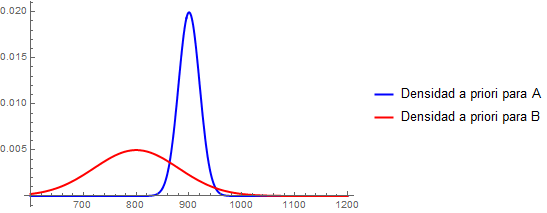
\includegraphics[width=0.6\textwidth]{imagenes4/apriori.png}
    \end{figure}
    \begin{figure}[H]
        \centering
        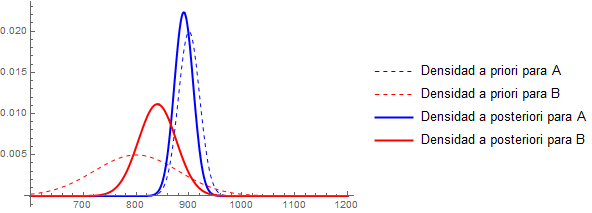
\includegraphics[width=0.6\textwidth]{imagenes4/aposte2.png}
    \end{figure}
    Supogamos ahora que tenemos una muestra $\vec{y} = (y_1,\ldots,y_{100})$ y que $\overline{y} = 870$. Ahora tendríamos que
    \begin{align*}
        \theta_A | \vec{y} \sim N(871'2, 3'9), \quad \theta_B | \vec{y} \sim N(869'8, 3'995),
    \end{align*}
    \begin{figure}[H]
        \centering
        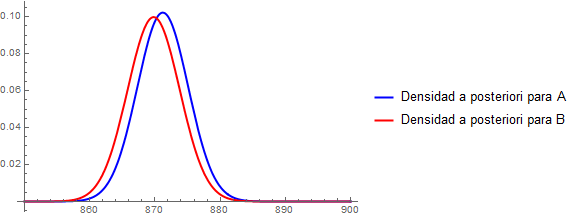
\includegraphics[width=0.6\textwidth]{imagenes4/aposte4.png}
    \end{figure}
    \begin{figure}[H]
        \centering
        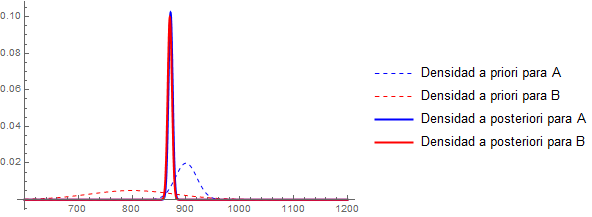
\includegraphics[width=0.6\textwidth]{imagenes4/aposte5.png}
    \end{figure}
\end{ejemplo}

\section{Inferencia Clásica vs. Inferencia Bayesiana}

\begin{align*}
     & \textbf{Clásicos}                          &  & \textbf{Bayesianos}                             \\
     & \text{Parámetros fijos}                    &  & \text{Parámetros variables}                     \\
     & \text{Probabilidad como frecuencia límite} &  & \text{Probabilidad como incertidumbre}          \\
     & \text{No incluye información previa}       &  & \text{Inclusión de información previa}          \\
     & \text{Estimadores de máxima verosimilitud} &  & \text{La estiamción es un problema de decisión} \\
     & \text{Intervalos de confianza}             &  & \text{Intervalos de credibilidad}               \\
     & \text{Método de muestreo muy importante}   &  & \text{El método de muestreo no importa}
\end{align*}

\subsubsection{Ventajas métodos bayesianos}

\begin{itemize}
    \item Permiten una inferencia más natural y útil que los métodos clásicos.
    \item Tienen una interpretación más directa que los intervalos de confianza, contrastes de hipótesis.
          clásicos y $p$-valor.
    \item Hacen uso de mayor cantidad de información disponible, lo que suele implicar resultados más consistentes que los obtenidos por el método clásico.
    \item Permiten ir actualizando resultados a medida que se incorpora nueva información.
    \item Permiten resolver problemas más complejos que los métodos clásicos.
    \item Son fundamentales para resolver problemas de decisión, mientras que los métodos clásicos están limitados a análisis estadíssticos que informan de la decisión sólo indirectamente.
    \item Son muy útiles en el caso de tamaños muestrales pequeños. No asumen mustras infinitas ni normalidad.
\end{itemize}

\subsubsection{Crísticas métodos bayesianos}
\begin{itemize}
    \item Los métodos bayesianos incorporan un elemento de subjetividad que no aparece de forma directa en los métodos clásicos.
    \item Las conclusiones dependenn de la selección de la distribución a priori.
    \item Se puede obtener resultados complejos que requiere del uso de métodos computacionales.
    \item En la práctica, la información extra que los métodos bayesianos utilizan es difícil de especificar de forma exacta.
\end{itemize}